
\documentclass[10pt,dvipdfmx]{beamer}
\usepackage{graphicx}
\DeclareGraphicsExtensions{.pdf}
\DeclareGraphicsExtensions{.eps}
\graphicspath{{out/}{out/tex/}{out/tex/gpl/}{out/tex/svg/}{out/tex/dot/}}
% \graphicspath{{out/}{out/tex/}{out/pdf/}{out/eps/}{out/tex/gpl/}{out/tex/svg/}{out/pdf/dot/}{out/pdf/gpl/}{out/pdf/img/}{out/pdf/odg/}{out/pdf/svg/}{out/eps/dot/}{out/eps/gpl/}{out/eps/img/}{out/eps/odg/}{out/eps/svg/}}
\usepackage{listings,jlisting}
\usepackage{fancybox}
\usepackage{hyperref}
\usepackage{color}

%% OpenMP section numbers
\newcommand{\sectionompparallel}{\href{https://www.openmp.org/spec-html/5.1/openmpse14.html\#x59-590002.6}{2.6}}
\newcommand{\sectionompdeterminenumthreads}{\href{https://www.openmp.org/spec-html/5.1/openmpsu40.html\#x60-600002.6.1}{2.6.1}}
\newcommand{\sectionompfor}{\href{https://www.openmp.org/spec-html/5.1/openmpsu48.html}{2.11.4}}
\newcommand{\sectioncanonicalloop}{\href{https://www.openmp.org/spec-html/5.1/openmpsu45.html\#x70-700002.11.1}{2.11.1}}
\newcommand{\sectionreductionclause}{\href{https://www.openmp.org/spec-html/5.1/openmpsu117.html\#x152-1760002.21.5.4}{2.21.5.4}}
\newcommand{\sectiondeclarereductionclause}{\href{https://www.openmp.org/spec-html/5.1/openmpsu117.html\#x152-1790002.21.5.7}{2.21.5.7}}

\newcommand{\sectionompdataenv}{\href{https://www.openmp.org/spec-html/5.1/openmpse29.html\#x147-1590002.21}{2.21}}
\newcommand{\sectionompgetnumthreads}{\href{https://www.openmp.org/spec-html/5.1/openmpsu121.html\#x160-1930003.2.2}{3.2.2}}
\newcommand{\sectionompgetmaxthreads}{\href{https://www.openmp.org/spec-html/5.1/openmpsu122.html\#x161-1940003.2.3}{3.2.3}}
\newcommand{\sectionompgetthreadnum}{\href{https://www.openmp.org/spec-html/5.1/openmpsu123.html\#x162-1950003.2.4}{3.2.4}}

%%%%%%%%%%%%%%%%%%%%%%%%%%% 
%%% themes
%%%%%%%%%%%%%%%%%%%%%%%%%%%
\usetheme{default} 
%% no navigation bar
% default boxes Bergen Boadilla Madrid Pittsburgh Rochester
%% tree-like navigation bar
% Antibes JuanLesPins Montpellier
%% toc sidebar
% Berkeley PaloAlto Goettingen Marburg Hannover Berlin Ilmenau Dresden Darmstadt Frankfurt Singapore Szeged
%% Section and Subsection Tables
% Copenhagen Luebeck Malmoe Warsaw

%%%%%%%%%%%%%%%%%%%%%%%%%%%
%%% innerthemes
%%%%%%%%%%%%%%%%%%%%%%%%%%%
% \useinnertheme{circles}       % default circles rectangles rounded inmargin

%%%%%%%%%%%%%%%%%%%%%%%%%%%
%%% outerthemes
%%%%%%%%%%%%%%%%%%%%%%%%%%%
% outertheme
% \useoutertheme{default}       % default infolines miniframes smoothbars sidebar sprit shadow tree smoothtree


%%%%%%%%%%%%%%%%%%%%%%%%%%%
%%% colorthemes
%%%%%%%%%%%%%%%%%%%%%%%%%%%
\usecolortheme{seahorse}
%% special purpose
% default structure sidebartab 
%% complete 
% albatross beetle crane dove fly seagull 
%% inner
% lily orchid rose
%% outer
% whale seahorse dolphin

%%%%%%%%%%%%%%%%%%%%%%%%%%%
%%% fontthemes
%%%%%%%%%%%%%%%%%%%%%%%%%%%
\usefonttheme{serif}  
% default professionalfonts serif structurebold structureitalicserif structuresmallcapsserif

%%%%%%%%%%%%%%%%%%%%%%%%%%%
%%% generally useful beamer settings
%%%%%%%%%%%%%%%%%%%%%%%%%%%
% 
\AtBeginDvi{\special{pdf:tounicode EUC-UCS2}}
% do not show navigation
\setbeamertemplate{navigation symbols}{}
% show page numbers
\setbeamertemplate{footline}[frame number]

%%%%%%%%%%%%%%%%%%%%%%%%%%%
%%% define some colors for convenience
%%%%%%%%%%%%%%%%%%%%%%%%%%%

\newcommand{\mido}[1]{{\color{green}#1}}
\newcommand{\mura}[1]{{\color{purple}#1}}
\newcommand{\ore}[1]{{\color{orange}#1}}
\newcommand{\ao}[1]{{\color{blue}#1}}
\newcommand{\aka}[1]{{\color{red}#1}}

\setbeamercolor{ex}{bg=cyan!20!white}

%%%%%%%%%%%%%%%%%%%%%%%%%%%
%%% how to typset code
%%%%%%%%%%%%%%%%%%%%%%%%%%%

\lstset{language = C,
numbers = left,
numberstyle = {\tiny \emph},
numbersep = 10pt,
breaklines = true,
breakindent = 40pt,
frame = tlRB,
frameround = ffft,
framesep = 3pt,
rulesep = 1pt,
rulecolor = {\color{blue}},
rulesepcolor = {\color{blue}},
flexiblecolumns = true,
keepspaces = true,
basicstyle = \ttfamily\scriptsize,
identifierstyle = ,
commentstyle = ,
stringstyle = ,
showstringspaces = false,
tabsize = 4,
escapechar=\@,
}

\title{計算科学概論 \\
  --- 高性能プログラミングと性能測定}
\institute{工学部 電子情報工学科 \\
  情報理工学系研究科 電子情報学専攻 \\
  情報基盤センター}
\author{田浦健次朗}
% \author{田浦健次朗 \\
%   {\scriptsize\url{https://www.eidos.ic.i.u-tokyo.ac.jp/~tau/lecture/cs_alliance/}} \\
%   $=$ \url{http://tinyurl.com/y8lmk9on} \\
% {\footnotesize (2018年5月4日18:01 講義日までに更新される可能性があります)}}
\date{}

\AtBeginSection[]
{
\begin{frame}
\frametitle{ロードマップ}
\tableofcontents[currentsection,currentsubsection]
\end{frame}
}

\AtBeginSubsection[]
{
\begin{frame}
\frametitle{ロードマップ}
\tableofcontents[currentsection,currentsubsection]
\end{frame}
}

\AtBeginSubsubsection[]
{
\begin{frame}
\frametitle{ロードマップ}
\tableofcontents[currentsection,currentsubsection]
\end{frame}
}

\begin{document}
\maketitle

%%%%%%%%%%%%%%%%%%%%%%%%%%%%%%%%%%
\begin{frame}
\frametitle{目標}

\begin{itemize}
\item 計算 \& 計算機の「性能」について理解して
\item 高性能プログラミングを実践 (Oakbridge CXで演習)

%\item {\footnotesize 第1回(4/20)「高性能計算機のアーキテクチャ」
%    と, その他の計算科学の題材の間をつなぐ}
\end{itemize}
\end{frame}

%%%%%%%%%%%%%%%%%%%%%%%%%%%%%%%%%% 
\begin{frame}
\frametitle{Contents}
\tableofcontents
\end{frame}

%%%%%%%%%%%%%%%%%
\section{計算科学で代表的なワークロード}
%%%%%%%%%%%%%%%%%

%%%%%%%%%%%%%%%%%
\begin{frame}[fragile]
\frametitle{計算科学で代表的なワークロード(1) --- 密行列}
\begin{itemize}
\item 例: 境界要素法, 深層学習
  \begin{center}
  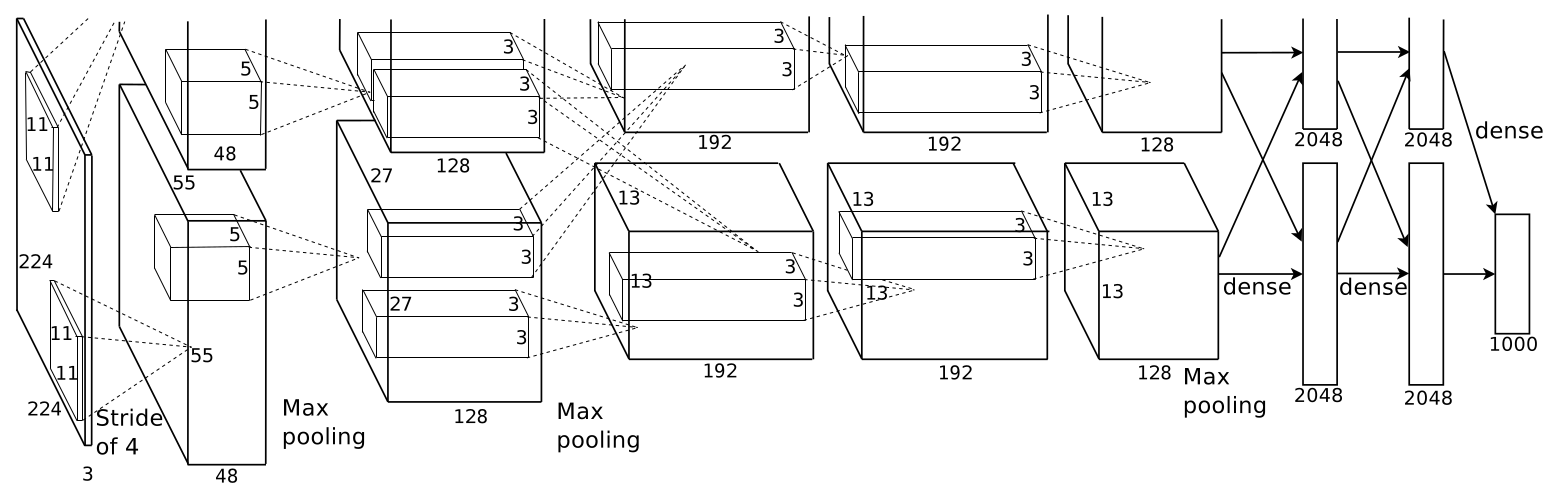
\includegraphics[width=0.6\textwidth]{out/pdf/img/alexnet.pdf}
  
  {\tiny Krizhevsky et al. ``ImageNet Classification with Deep Convolutional Neural Networks''}
  \end{center}

\item 計算カーネル: 行列・行列積
\begin{columns}
\begin{column}{0.5\textwidth}
\begin{lstlisting}
for (i = 0; i < M; i++)    
  for (j = 0; j < N; j++)    
    for (k = 0; k < K; k++)
      C(i,j) += A(i,k) * B(k,j); 
\end{lstlisting}
\end{column}
\begin{column}{0.5\textwidth}
\includegraphics[width=\textwidth]{out/pdf/svg/mm0.pdf}
\end{column}
\end{columns}
\end{itemize}
\end{frame}

%%%%%%%%%%%%%%%%%
\begin{frame}[fragile]
\frametitle{計算科学で代表的なワークロード(2) --- 疎行列}

\begin{itemize}
\item 例: 不規則格子での差分法や有限要素法

  \begin{center}
  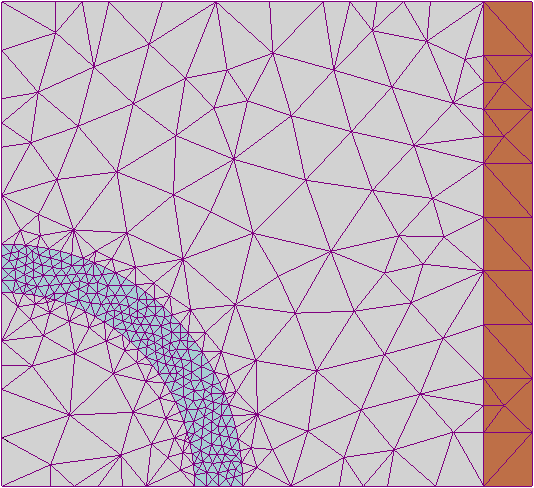
\includegraphics[width=0.35\textwidth]{out/pdf/img/Example_of_2D_mesh.pdf}

  {\tiny www.wikipedia.org}
  \end{center}
  
\item 計算カーネル: 疎行列ベクトル積
\begin{lstlisting}
for (i = 0; i < M; i++) {
  y[i] = 0;
  for (idx = start[i]; idx < start[i+1]; idx++) {
    y[i] += A[idx] * x[J[idx]];
  }
}
\end{lstlisting}

% \includegraphics[width=0.5\textwidth]{out/pdf/svg/spmv.pdf}

\end{itemize}
\end{frame}

%%%%%%%%%%%%%%%%%
\begin{frame}[fragile]
\frametitle{計算科学で代表的なワークロード(3) --- $N$体問題}

\begin{itemize}
\item 例: 分子動力学, 天文, 流体, \ldots
  \begin{center}
  
\includegraphics[width=0.4\textwidth]{out/pdf/img/Galaxy_cluster_sim.pdf}

  {\tiny www.wikipedia.org}
\end{center}

\item 計算カーネル: 直接計算, 多重極展開

\item 重力の直接計算カーネル
\begin{lstlisting}
for (i = 0; i < n; i++) {
  for (j = 0; j < n; j++) {
    if (i != j) {
      dx = p[j].pos - p[i].pos;
      r = |dx|;
      p[i].acc += p[j].m * dx / (r * r * r);
    }
  }
}
\end{lstlisting}
\end{itemize}
\end{frame}

%%%%%%%%%%%%%%%%%
\begin{frame}
\frametitle{計算科学で代表的なワークロード(4) --- モンテカルロ法}

\begin{itemize}
\item 例: 統計物理, 機械学習, あらゆる期待値計算, \ldots

  
\end{itemize}
\end{frame}


%%%%%%%%%%%%%%%%%
\section{計算機の「性能」}
%%%%%%%%%%%%%%%%%

%%%%%%%%%%%%%%%%%
\begin{frame}
  \frametitle{計算機の「性能」}
  \begin{itemize}
  \item<1-> プロセッサ(CPUやGPU)の性能は普通\ao{「○○ FLOPS」}と表現され,
    1秒に実行可能な最大の\ao{浮動小数点演算数}を表す
    \begin{itemize}
    \item<2-> \ao{FLOPS} $=$ \ao{FL}oating point \ao{O}perations
      \ao{P}er \ao{S}econd
    \item<3-> 例えば 10 GFLOPS $=$ 1 $\times 10^{10}$ FLOPS
    \item<3->
      K $= 10^3$,
      M $= 10^6$,
      G $= 10^9$,
      T $= 10^{12}$,
      P $= 10^{15}$,
      E $= 10^{18},$ \ldots
    \end{itemize}
  \item<4-> ちなみに \ao{flop (小文字)}は
    \ao{floating point operation}の意味で使われる事が多い
    \begin{itemize}
    \item 100 flops $=$ 100回の浮動小数点演算
    \item 100 FLOPS $=$ 毎秒100回の浮動小数点演算
    \end{itemize}
  \end{itemize}
\end{frame}

%%%%%%%%%%%%%%%%%
\begin{frame}
  \frametitle{今時のCPU/GPUの「性能」}
  \begin{itemize}
  \item 単位: TFLOPS
    
  \item []
    {\small
\begin{tabular}{|l|r|r|r|}\hline
                      & 倍精度 & 単精度 & 消費電力 \\\hline
NVIDIA Tesla P100     & 5.0    & 10.0   & $\approx$ 300W \\
NVIDIA Tesla V100     & 7.5    & 15.0   & $\approx$ 300W \\    
NVIDIA Tesla A100 PCIe (*) & 9.7    & 19.5   & $\approx$ 300W \\    
NVIDIA Tesla H100 PCIe (*) & 30.0  & 60.0   & $\approx$ 350W \\    
Intel Knights Landing & 3.0    & 6.0    & $\approx$ 250W \\
Intel Broadwell E5-2695 v4 & 0.6 & 1.2  & $\approx$ 120W \\
Intel Cascade Lake Platinum 8280 (**) & 2.4 & 4.8  & $\approx$ 205W \\
Intel IceLake Platinum 8380 & 2.9 & 5.9  & $\approx$ 270W \\\hline
\end{tabular}}
\item (*) Tensor Core (行列積用の特殊命令)を使わない場合
\item (**) Oakbridge CX
\end{itemize}
\end{frame}

%%%%%%%%%%%%%%%%%
\begin{frame}
  \frametitle{「性能」について知っておかねばならない事}
  \begin{itemize}
  \item<1-> このCPU/GPUの「性能」が○○ FLOPSというのは,
    割と多くのアプリケーションで自然にそのくらい(例: 6〜7割)
    の性能が出る, ということを意味していない
  \item<2-> 常に最大性能が出るわけじゃないのは当たり前, と思うでしょうが,
    そのギャップの大きさには驚き, 怒りすら覚えるかも知れません
  \item<3-> 不都合な真実?
  \end{itemize}
\end{frame}

%%%%%%%%%%%%%%%%%
\begin{frame}[fragile]
  \frametitle{不都合な真実 --- 密行列積の場合}
  \begin{itemize}
  \item 以下の密行列積コード:
\begin{columns}
\begin{column}{0.5\textwidth}
\begin{lstlisting}
for (long i = 0; i < M; i++) {
  for (long j = 0; j < N; j++) {
    for (long k = 0; k < K; k++) {
      C(i,j) += A(i,k) * B(k,j);
    }
  }
}
\end{lstlisting}
\end{column}
\begin{column}{0.5\textwidth}
\includegraphics[width=\textwidth]{out/pdf/svg/mm0.pdf}
\end{column}
\end{columns}

% \item をReedbushの,「性能」 1.2 TFLOPSのプロセッサIntel Broadwell E5-2695 v4 (Reedbushの計算ノード)で実行したときの性能は?
\item を「性能」 4.8 TFLOPSのプロセッサ
  Intel Xeon Platinum 8280 CPU (Oakbridge CXの計算ノードのプロセッサ)
  で実行したときの性能は?
\end{itemize}
\end{frame}

%%%%%%%%%%%%%%%%%
\begin{frame}[fragile]
\frametitle{実際の結果}
\begin{lstlisting}
A = 1000 x 1000 (4000000 bytes)
B = 1000 x 1000 (4000000 bytes)
C = 1000 x 1000 (4000000 bytes)
repeat C += A * B 1 times
2000000000 flops, total 12000000 bytes
2762354648 clocks
1.025528 sec
0.724 flops/clock
@\aka{\texttt{1.950215 GFLOPS}}@
2.762 clocks/muladd
OK: max relative error = 0.000000
\end{lstlisting}

\begin{itemize}
\item CPUの最大性能 4.8 TFLOPSと比べると約\aka{1/2461} (!)
  
\item ちなみに計算ノードには同CPUが2個積まれているので,
  計算ノードの最大性能は9.6 TFLOPS
\end{itemize}
\end{frame}

%%%%%%%%%%%%%%%%%
\begin{frame}
  \frametitle{最大「性能」の真実}
  \begin{itemize}
  \item<1-> プロセッサの性能を決めているのは, 
    1クロックに実行できる命令数
  \end{itemize}
  \begin{columns}[t]
    \begin{column}{0.6\textwidth}
      \begin{itemize}
      \item<2-> ざっくり言えば, 1クロックに,
        \begin{itemize}
        \item 浮動小数点命令が○個
        \item $+$ 整数演算が○個
        \item $+$ load命令が○個
        \item $+$ store命令が○個,
        \item \ldots みたいな
        \end{itemize}

      \item<3-> 最大「性能」は以下の掛け算の結果に過ぎない:
        \[
          {\small\begin{array}{ll}
                   & \mbox{1浮動小数点命令あたりの演算数} \\
            \times & \mbox{1クロックに実行できる浮動小数点命令数} \\
            \times & \mbox{クロック周波数(秒あたりのクロック数)} \\
            \times & \mbox{コア数}
          \end{array}}
        \]
      \end{itemize}
    \end{column}

    \begin{column}{0.4\textwidth}
      \begin{center}
        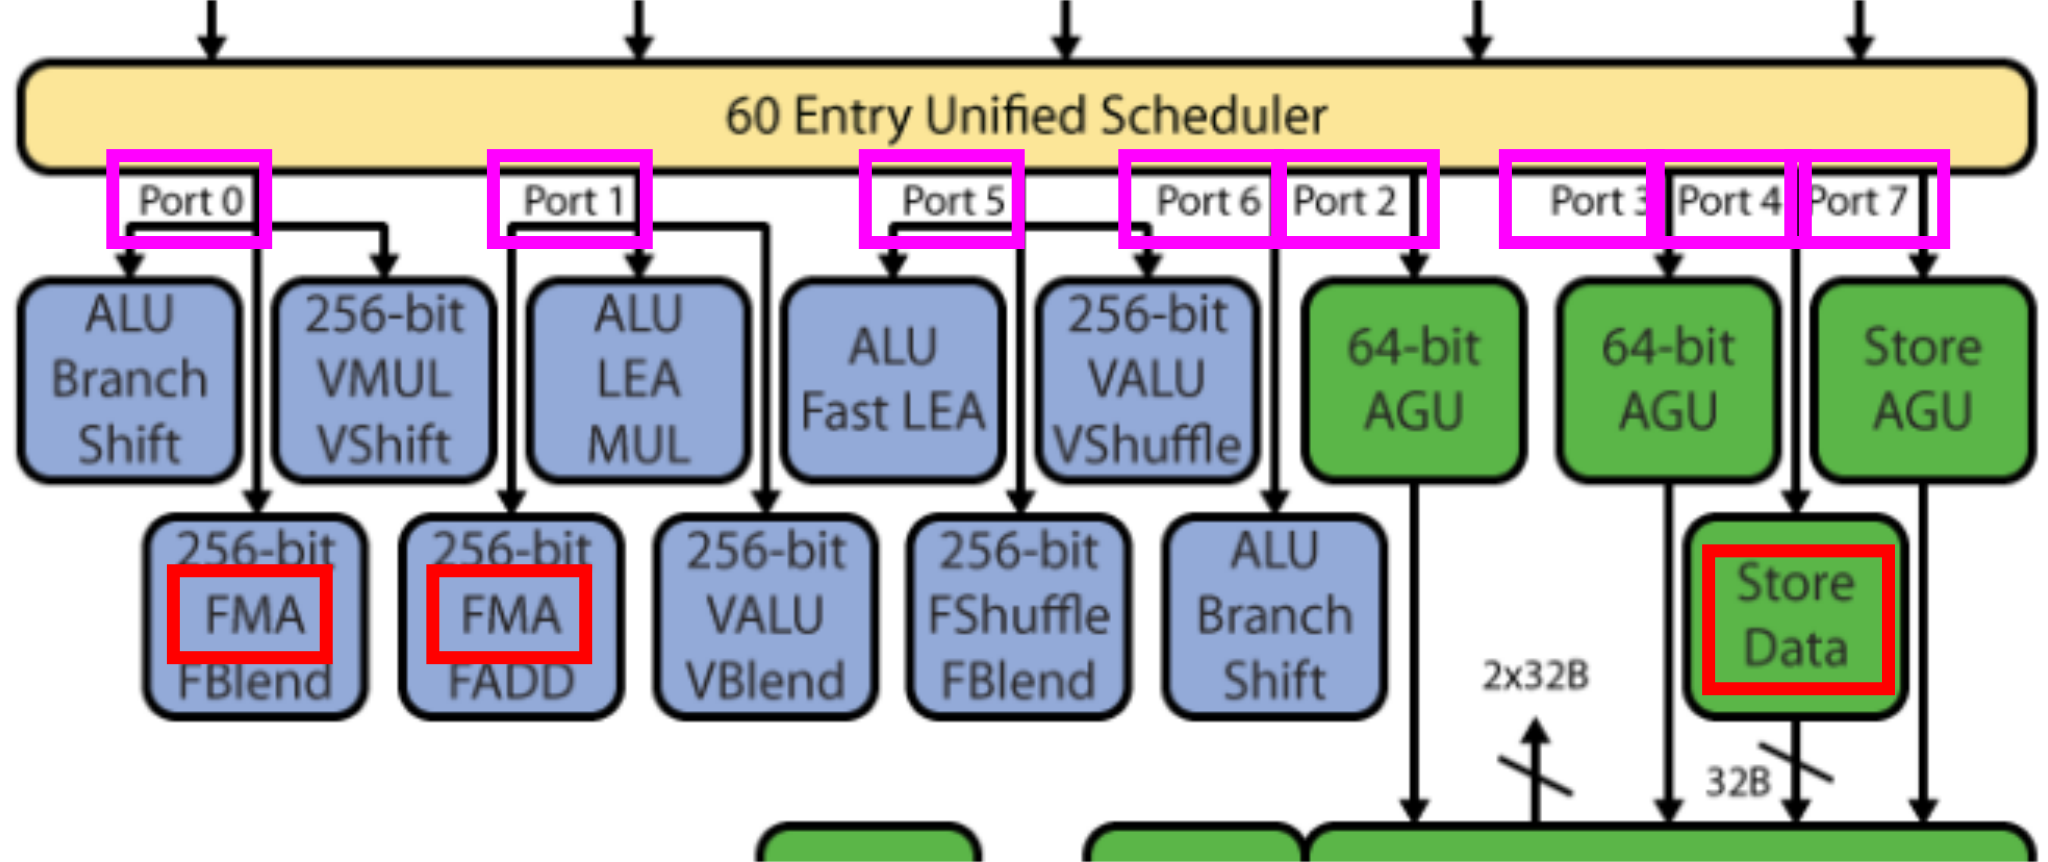
\includegraphics[width=\textwidth]{out/pdf/svg/haswell_ports.pdf}
        
        {\tiny source: \url{http://www.realworldtech.com/haswell-cpu/}}
      \end{center}
    \end{column}
  \end{columns}
\end{frame}


%%%%%%%%%%%%%%%%%
\iffalse
\begin{frame}
  \frametitle{例: Intel Broadwell (E5-2695 v4 2.10 GHz)の場合}
\begin{itemize}
\item 単精度 (32 bit) 浮動小数点数の場合:
  \[
    \begin{array}{ll}
      \only<1->{& \phantom{\mbox{1クロックに実行できる浮動小数点命令数}}} \\
      \only<2->{& \mbox{1浮動小数点命令あたりの演算数}} \\
      \only<3->{\times & \mbox{1クロックに実行できる浮動小数点命令数}} \\
      \only<4->{\times & \mbox{クロック周波数(秒あたりのクロック数)}} \\
      \only<5->{\times & \mbox{コア数}} \\
      \only<2->{= & 16 \mbox{ flops}}
                    \only<3->{\times 2}
                    \only<4->{\times 2.1 \mbox{ GHz (1/sec)}}
                    \only<5->{\times 18} \\
      \only<6->{= & \ao{1209.6 \mbox{ GFLOPS} \; (1.2 \mbox{ TFLOPS})}}
    \end{array}
  \]
\end{itemize}

\begin{columns}
\begin{column}{0.5\textwidth}
\begin{itemize}
\item<7-> 注: 倍精度 (64 bit)浮動小数点数の場合:
  1クロックに実行できる浮動小数点命令数 $=$ 8 となる以外は同じ
\end{itemize}
\end{column}
\begin{column}{0.5\textwidth}
  \includegraphics[width=0.90\textwidth]{out/pdf/svg/diagram_multisocket_and_core.pdf} 
\end{column}
\end{columns}
\end{frame}
\fi

%%%%%%%%%%%%%%%%%
\begin{frame}
  \frametitle{例: Cascade Lake (Intel Platinum 8280)の場合}
\begin{itemize}
\item 単精度 (32 bit) 浮動小数点数の場合:
  \[
    \begin{array}{ll}
      \only<1->{& \phantom{\mbox{1クロックに実行できる浮動小数点命令数}}} \\
      \only<2->{& \mbox{1浮動小数点命令あたりの演算数}} \\
      \only<3->{\times & \mbox{1クロックに実行できる浮動小数点命令数}} \\
      \only<4->{\times & \mbox{クロック周波数(秒あたりのクロック数)}} \\
      \only<5->{\times & \mbox{コア数}} \\
      \only<2->{= & 32 \mbox{ flops}}
                    \only<3->{\times 2}
                    \only<4->{\times 2.7 \mbox{ GHz (1/sec)}}
                    \only<5->{\times 28} \\
      \only<6->{= & \ao{4838.4 \mbox{ GFLOPS} \; (4.8 \mbox{ TFLOPS})}}
    \end{array}
  \]
\end{itemize}

\begin{columns}
\begin{column}{0.5\textwidth}
\begin{itemize}
\item<7-> 注: 倍精度 (64 bit)浮動小数点数の場合:
  1クロックに実行できる浮動小数点命令数 $=$ 8 となる以外は同じ
\end{itemize}
\end{column}
\begin{column}{0.5\textwidth}
  \includegraphics[width=0.90\textwidth]{out/pdf/svg/diagram_multisocket_and_core.pdf} 
\end{column}
\end{columns}
\end{frame}


%%%%%%%%%%%%%%%%%
\iffalse
\begin{frame}
  \frametitle{1浮動小数点命令あたりの演算数について}
  \begin{itemize}
  \item<1-> Intel Broadwellは\ao{256 bit}幅のレジスタ (\ao{SIMDレジスタ})を持つ
    
  \item<2-> 256 bit (32 bytes) $=$ 単精度 (32 bit / 4 bytes))
    浮動小数点数が\ao{8つ}
    \begin{center}
    \includegraphics[width=0.6\textwidth]{out/pdf/svg/simd_reg.pdf}
    \end{center}

  \item<3-> 乗算と加算を同時に行う命令 (fmadd) があり,
    それを使うと1命令で$8 \times 2 = \ao{16}$演算ということになる
    \[ c = a * b + c \]

  \item<4->
    同じ\ao{SIMDレジスタ}で倍精度(64 bit / 8 bytes)数4つを保持することもできる
    (したがってfmaddの演算数$=$8)
  \end{itemize}
\end{frame}
\fi

%%%%%%%%%%%%%%%%% 
\begin{frame}
  \frametitle{1浮動小数点命令あたりの演算数について}
  \begin{itemize}
  \item<1-> Intel Cascade Lakeは\ao{512 bit}幅のレジスタ (\ao{SIMDレジスタ})を持つ
    
  \item<2-> 512 bit (64 bytes) $=$ 単精度 (32 bit / 4 bytes))
    浮動小数点数が\ao{16つ}
    \begin{center}
    \includegraphics[width=0.6\textwidth]{out/pdf/svg/simd_reg16.pdf}
    \end{center}

  \item<3-> 乗算と加算を同時に行う命令 (fmadd) があり,
    それを使うと1命令で$16 \times 2 = \ao{32}$演算ということになる
    \[ c = a * b + c \]

  \item<4->
    同じ\ao{SIMDレジスタ}で倍精度(64 bit / 8 bytes)数8つを保持することもできる
    (したがってfmaddの演算数$=$16)
  \end{itemize}
\end{frame}

%%%%%%%%%%%%%%%%% 
\begin{frame}
  \frametitle{知ってしまった真実}
  \begin{itemize}
  \item[]
    \begin{tabular}{llrr}
    fmadd命令を使わ(え)ない  & $\rightarrow$ & \aka{1/2} & \aka{(50.0\%)} \\
      SIMD命令を使わ(え)ない & $\rightarrow$ & \aka{1/16} & \aka{(6.25\%)} \\
      並列化して(でき)いない & $\rightarrow$ & \aka{1/28} & \aka{(3.57\%)} \\
      どれも使って(え)ない   & $\rightarrow$ & \aka{1/896} & \aka{(0.11\%)}
    \end{tabular}
  \item $\Rightarrow$ 最大性能に近い性能は, 相当限られた状況でのみ目にできる
  \item これらを意識せずにプログラムを書いたら言語処理系がそれらを勝手に使ってくれる,
    というのが理想だがなかなかそうはなっていない
  \end{itemize}
\end{frame}

\iffalse
%%%%%%%%%%%%%%%%% 
\begin{frame}
  \frametitle{NVIDIA GPUの場合}
  \begin{itemize}
  \item Deep Learning
  \end{itemize}
\end{frame}

%%%%%%%%%%%%%%%%% 
\begin{frame}
  \frametitle{Intel Knights Millの場合}
  \begin{itemize}
  \item Deep Learningで4倍
  \end{itemize}
\end{frame}
\fi

%%%%%%%%%%%%%%%%%
\section{高性能プログラミングの実践}
%%%%%%%%%%%%%%%%%

%%%%%%%%%%%%%%%%% 
\begin{frame}
  \frametitle{高性能「プログラミング」とは}
  \begin{enumerate}
  \item<1-> ワークロードを見て, 
  \item<2-> 「出せるはずの(近似)性能」を理解して, 
  \item<3-> 正しく道具(SIMD, 並列)を取り出し, 
  \item<4-> それに近い性能を出す
  \end{enumerate}
\end{frame}


\iffalse
%%%%%%%%%%%%%%%%% 
\begin{frame}
  \frametitle{ワークロードを見る}
  \begin{itemize}
  \item 例: 行列積
  \item $(M,K) \times (K,N)$ の行列積
  \item $MNK$ 乗算 $+$ $MNK$加算
  \end{itemize}
\end{frame}

  
  %%%%%%%%%%%%%%%%%
\begin{frame}
  \frametitle{出せるはずの(近似)性能}
  \begin{itemize}
  \item プロセッサの演算スループットから来る限界
    \begin{itemize}
    \item 例: 毎クロック浮動小数点乗算,加算,FMADD命令が2個, load命令が2個, store命令が1個, etc.
    \end{itemize}
  \item メモリアクセスのスループットから来る限界
  \item 演算およびメモリアクセスの遅延
    $+$依存関係から来る限界
  \end{itemize}
\end{frame}

%%%%%%%%%%%%%%%%% 
\begin{frame}
  \frametitle{正しく道具(SIMD, 並列)を取り出す}
  \begin{itemize}
  \item どうプログラムを書けばSIMD化, 並列化されるのかを覚える
  \item 言語処理系(コンパイラ)がよろしくやってくれるのか,
    自分で書かないといけないのか

  \item C/C++言語で書く限り,
    \begin{itemize}
    \item 並列化: 「やってくれない」と割り切るので良い
    \item SIMD化: たまにはやってくれるけど
    \end{itemize}
  \end{itemize}
\end{frame}

  %%%%%%%%%%%%%%%%%
\begin{frame}[fragile]
\frametitle{まずは役に立たない例}
\begin{itemize}
\item 道具の紹介を兼ね, ともかくCPUの限界性能を出してみる
\item []
  \lstinputlisting[firstline=2,lastline=5]{../prog/triv/triv0.h}
\item $n$加算$+n$乗算
\item 期待時間(クロック数)は?
\end{itemize}
\end{frame}

%%%%%%%%%%%%%%%%% 
\begin{frame}[fragile]
\frametitle{SIMD化}
\begin{itemize}
\item 以下で\texttt{float} (単精度(4バイト)浮動小数点数型)を8つ並べた(32バイト)
  SIMD型を定義
  \lstinputlisting[firstline=1,lastline=1]{../prog/triv/triv1.h}
\item これに対して演算をするとそれがSIMD演算になる
  \lstinputlisting[firstline=4,lastline=7]{../prog/triv/triv1.h}
\end{itemize}
\end{frame}

%%%%%%%%%%%%%%%%% 
\begin{frame}
\frametitle{これだけでは最大性能が出ない理由}
\begin{itemize}
\item fmadd命令の遅延
\end{itemize}
\end{frame}

%%%%%%%%%%%%%%%%% 
\begin{frame}[fragile]
\frametitle{役に立たない例でCPUの限界 ---  OpenMPでマルチコア並列化}
\begin{itemize}
\item []
  \begin{lstlisting}
    for (i = 0; i < n; i++) {
      
    }
  \end{lstlisting}
\end{itemize}
\end{frame}

%%%%%%%%%%%%%%%%% 
\begin{frame}[fragile]
\frametitle{役に立たない例でCPUの限界 --- MPIで複数ノード並列化}
\begin{itemize}
\item []
  \begin{lstlisting}
    for (i = 0; i < n; i++) {
      
    }
  \end{lstlisting}
\end{itemize}
\end{frame}
\fi

%%%%%%%%%%%%%%%%%
\begin{frame}
  \frametitle{以降のロードマップ}
  \begin{itemize}
  \item 実例に沿って各要素を説明
  \item ワークロード
    \begin{itemize}
    \item 密行列積
    \item $N$体問題の直接法カーネル部分
    \end{itemize}
  \item それぞれのツールを使うための「プログラミング」
    \begin{itemize}
    \item \ao{SIMD化} --- ベクタ型, intrinsics
    \item \ao{マルチコア並列化} --- OpenMP parallel/for pragma
    \item \ao{複数ノード並列化} --- MPI (時間切れの予定)
    \end{itemize}
  \item 思想・哲学
    \begin{itemize}
    \item 速くなったという結果より,
      何が起きているかをしっかり理解するのが大事
    \item つまり,
      何が起きているかを調べる方法を覚えるのが大事
    \item コンパイラが出したコードを見る, 測定する
    \end{itemize}
  \end{itemize}
\end{frame}

%%%%%%%%%%%%%%%%%
\subsection{ワークロード}
%%%%%%%%%%%%%%%%%


%%%%%%%%%%%%%%%%%
\begin{frame}[fragile]
\frametitle{想定ワークロード(1) --- 密行列積}
\begin{lstlisting}
for (i = 0; i < M; i++) {
 for (j = 0; j < N; j++) {
  real c = 0.0;
  for (k = 0; k < K; k++) {
   c += A(i,k) * B(k,j);
  }
  C(i,j) += c;
 }
}
\end{lstlisting}
\end{frame}

%%%%%%%%%%%%%%%%%
\begin{frame}[fragile]
\frametitle{想定ワークロード(2) --- $N$体問題}
\begin{lstlisting}
real interact_all(long n, particle * p) {
  for (i = 0; i < n; i++) {
    for (j = 0; j < n; j++) {
      if (i != j) {
        dx = p[j].pos - p[i].pos; // (x,y,z)のベクトル
        r = |dx|; // (x*x+y*y+z*z)^{1/2}
        p[i].acc += p[j].m * dx / (r * r * r);
      }
    }
  }
}
\end{lstlisting}
\end{frame}

%%%%%%%%%%%%%%%%%
\subsection{SIMD化}
%%%%%%%%%%%%%%%%%

%%%%%%%%%%%%%%%%%
\begin{frame}
  \frametitle{SIMD化基礎}
  \begin{itemize}
  \item \ao{SIMD}命令$=$ \ao{S}ingle \ao{I}nstruction \ao{M}ultiple \ao{D}ata命令
  \item ひとつの命令で複数のデータに同時に(同じ)演算

    \begin{center}
    \includegraphics[width=0.9\textwidth]{out/pdf/svg/simd_reg_add16.pdf}
    \end{center}
    
    \begin{itemize}
    \item CPUにとっては, 命令デコードやディスパッチのオーバーヘッドを減らし,
      低消費電力で最大性能を稼ぐ手段
    \end{itemize}
  \item \ao{注:} SIMD命令(化)のことをしばしば\ao{ベクトル}命令(化)と言う
  \item 昔のベクトル計算機におけるベクトル命令とは違うが,
    考え方は似ているので, もはや区別しなくても平気(?)
  \end{itemize}
\end{frame}

%%%%%%%%%%%%%%%%%%%%%%%%%%%%%%%%%% 
%%%%%%%%%%%%%%%%%%%%%%%%%%%%%%%%%% 
\subsubsection{SIMD命令}
%%%%%%%%%%%%%%%%%%%%%%%%%%%%%%%%%% 
%%%%%%%%%%%%%%%%%%%%%%%%%%%%%%%%%% 

%%%%%%%%%%%%%%%%%%%%%%%%%%%%%%%%%% 
\begin{frame}
  \frametitle{IntelのSIMD命令概要}
  \begin{itemize}
  \item Intelは長きに渡り, 命令セットを拡張してSIMD命令を増やしてきた(今も増えている)
  \item ひとつのSIMD命令で扱えるbit幅も増え続けている
  \item 命令セット名 (括弧内はSIMDのbit幅):
    \ao{MMX} (64) $\rightarrow$ \ao{SSE3} (128) $\rightarrow$ \ao{SSE4} (128)
    $\rightarrow$ \ao{AVX} (256)
    $\rightarrow$ \ao{AVX2} (256)
    $\rightarrow$ \ao{AVX-512} (512)
\iffalse
  \item ReedbushのCPUは Broadwell というマイクロアーキテクチャで \ao{AVX2}
    までをサポート
\fi
  \item Oakbridge CXのCPUは Cascade Lake というマイクロアーキテクチャで \ao{AVX-512}
    までをサポート
    
  \item 自分で書ける必要はないが「どんなコードがSIMD化できるのか」
    を知る, 無事SIMD化できたかを判断できるようになる必要がある
  \end{itemize}
  
\end{frame}

%%%%%%%%%%%%%%%%%%%%%%%%%%%%%%%%%%
\iffalse
\begin{frame}
  \frametitle{いくつかのAVX命令 (アセンブリ言語)}

\begin{center}
{\footnotesize
\begin{tabular}{|l|l|l|}\hline
演算   & 表記                         & 意味(C風表記で) \\\hline
乗算   & {\tt \ao{vmulps} \%ymm0,\%ymm1,\%ymm2} & {\tt ymm2 = ymm1 * ymm0} \\
加算   & {\tt \ao{vaddps} \%ymm0,\%ymm1,\%ymm2} & {\tt ymm2 = ymm1 + ymm0} \\
乗加算 & {\tt \ao{vfmadd132ps} \%ymm0,\%ymm1,\%ymm2} & {\tt ymm2 = ymm0*ymm2+ymm1} \\
ロード  & {\tt \ao{vmovups} 400(\%rax),\%ymm0}   & {\tt ymm0 = *(rax+400)} \\
ストア  & {\tt \ao{vmovups} \%ymm0,400(\%rax)}   & {\tt *(rax+400) = ymm0} \\
\hline
\end{tabular}}
\end{center}

\begin{itemize}

\item \texttt{ymm0}, \texttt{ymm1} \ldots SIMDレジスタ (通常ymmレジスタ)
  \begin{itemize}
  \item 8個の単精度浮動小数点数(Cの\texttt{float}),
    4個の倍精度浮動小数点数(Cの\texttt{double})を保持できる
  \end{itemize}
\item \texttt{ymm0}, \ldots , \texttt{ymm15} まで 16個ある 
\item {\tt XXXX\ao{ps}}は{\em \ao{p}acked \ao{s}ingle precision}の略で,
  単精度用のSIMD命令であることを示す
\end{itemize}
\end{frame}
\fi

%%%%%%%%%%%%%%%%%%%%%%%%%%%%%%%%%% 
\begin{frame}
  \frametitle{いくつかのAVX-512命令 (アセンブリ言語)}

\begin{center}
{\footnotesize
\begin{tabular}{|l|l|l|}\hline
演算   & 表記                         & 意味(C風表記で) \\\hline
乗算   & {\tt \ao{vmulps} \%zmm0,\%zmm1,\%zmm2} & {\tt zmm2 = zmm1 * zmm0} \\
加算   & {\tt \ao{vaddps} \%zmm0,\%zmm1,\%zmm2} & {\tt zmm2 = zmm1 + zmm0} \\
乗加算 & {\tt \ao{vfmadd132ps} \%zmm0,\%zmm1,\%zmm2} & {\tt zmm2 = zmm0*zmm2+zmm1} \\
ロード  & {\tt \ao{vmovups} 400(\%rax),\%zmm0}   & {\tt zmm0 = *(rax+400)} \\
ストア  & {\tt \ao{vmovups} \%zmm0,400(\%rax)}   & {\tt *(rax+400) = zmm0} \\
\hline
\end{tabular}}
\end{center}

\begin{itemize}

\item \texttt{zmm0}, \texttt{zmm1} \ldots SIMDレジスタ (通常zmmレジスタ)
  \begin{itemize}
  \item 16個の単精度浮動小数点数(Cの\texttt{float}),
    8個の倍精度浮動小数点数(Cの\texttt{double})を保持できる
  \end{itemize}
\item \texttt{zmm0}, \ldots , \texttt{zmm31} まで 32個ある 
\item {\tt XXXX\ao{ps}}は{\em \ao{p}acked \ao{s}ingle precision}の略で,
  単精度用のSIMD命令であることを示す
\end{itemize}
\end{frame}


%%%%%%%%%%%%%%%%%%%%%%%%%%%%%%%%%%
\iffalse
\begin{frame}
  \frametitle{ロード・ストア命令について}
\begin{center}
{\footnotesize
\begin{tabular}{|l|l|l|}\hline
ロード     & {\tt \ao{vmovaps} 400(\%rax),\%ymm0}   & {\tt ymm0 = *(rax+400)} \\
ストア     & {\tt \ao{vmovaps} \%ymm0,400(\%rax)}   & {\tt *(rax+400) = ymm0} \\
\hline
\end{tabular}}
\begin{itemize}
\item \texttt{\%rax}は汎用レジスタで64 bitの整数(アドレス)を1つ保持できる
\item \texttt{400(\%rax)}は (\texttt{\%rax} $+$ 400) 番地を指定する記法
\item {\tt vmovaps} ({\tt vmovups}もある)は, 
  指定したアドレスから\ao{連続した256 bit (32バイト)}をアクセスする

  \begin{center}
    \includegraphics[width=0.9\textwidth]{out/pdf/svg/simd_reg_load.pdf}
  \end{center}
  
\item AVX2以降は,
  バラバラのアドレスをアクセスする命令(gather, scatter)もあるが, 省略
\end{itemize}
\end{center}
\end{frame}
\fi

%%%%%%%%%%%%%%%%%%%%%%%%%%%%%%%%%% 
\begin{frame}
  \frametitle{ロード・ストア命令について}
\begin{center}
{\footnotesize
\begin{tabular}{|l|l|l|}\hline
ロード     & {\tt \ao{vmovups} 40(\%rax),\%zmm1}   & {\tt zmm1 = *(rax+40)} \\
ストア     & {\tt \ao{vmouups} \%zmm1,40(\%rax)}   & {\tt *(rax+40) = zmm1} \\
\hline
\end{tabular}}
\begin{itemize}
\item \texttt{\%rax}は汎用レジスタで64 bitの整数(アドレス)を1つ保持できる
\item \texttt{32(\%rax)}は (\texttt{\%rax} $+$ 32) 番地を指定する記法
\item {\tt vmovups} は, 
  指定したアドレスから\ao{連続した512 bit (64バイト)}をアクセスする

  \begin{center}
    \includegraphics[width=0.9\textwidth]{out/pdf/svg/simd_reg_load16.pdf}
  \end{center}
  
\item AVX2以降は,
  バラバラのアドレスをアクセスする命令(gather, scatter)もあるが, 省略
\end{itemize}
\end{center}
\end{frame}



%%%%%%%%%%%%%%%%%%%%%%%%%%%%%%%%%% 
\iffalse
\begin{frame}
  \frametitle{SIMD命令と非SIMD (スカラ)命令}
  \begin{itemize}
  \item 似て非なる命令たち
  \item SIMD版 (\texttt{\ao{...p.}}) vs. スカラ版 (\texttt{\ao{...s.}})
  \item 同じSIMDでも256 bit版 (ymm)と128 bit版 (xmm)
  \end{itemize}
\begin{center}
{\footnotesize
\begin{tabular}{|l|c|c|c|c|}\hline
                     & 演算対象 & SIMD    & 幅     & ISA \\
                     &          & /スカラ? & (bits) &     \\
\hline
{\tt \ao{v}mulps \%ymm0,\%ymm1,\%ymm2} & 8 SPs & vector     & 256  & AVX \\
{\tt vmul\ao{pd} \%ymm0,\%ymm1,\%ymm2} & 4 DPs & vector     & 256  & AVX \\
{\tt  mulps \ao{\%xmm0},\%xmm1} & 4 SPs     & vector        & 128  & SSE \\
{\tt  mulpd \%xmm0,\%xmm1} & 2 DPs     & vector        & 128  & SSE \\
{\tt  mul\ao{ss} \%xmm0,\%xmm1} & 1 SP      & scalar        & (32) & SSE \\
{\tt  mul\ao{sd} \%xmm0,\%xmm1} & 1 DP      & scalar        & (64) & SSE \\
{\tt  vfmadd132\ao{ss} \%ymm0,\%ymm1,\%ymm2} & 1 SP & scalar   & (32) & AVX \\
\hline
\end{tabular}}
\end{center}

\begin{itemize}
\item \ldots ps : \ao{\em p}acked \ao{\em s}ingle precision
\item \ldots pd : \ao{\em p}acked \ao{\em d}ouble precision
\item xmm0, \ldots , xmm15 : 128 bit SSE registers 
  (xmm$i$は, 実はymm$i$の下半分)
\end{itemize}
\end{frame}
\fi

%%%%%%%%%%%%%%%%%%%%%%%%%%%%%%%%%%
\begin{frame}
  \frametitle{SIMD命令と非SIMD (スカラ)命令}
  \begin{itemize}
  \item 似て非なる命令たち
  \item SIMD版 (\texttt{\ao{...p.}}) vs. スカラ版 (\texttt{\ao{...s.}})
  \item SIMD版も512 bit版 (zmm), 256 bit版 (ymm), 128 bit版 (xmm)
  \end{itemize}
\begin{center}
{\footnotesize
\begin{tabular}{|l|c|c|c|c|}\hline
                     & 演算対象 & SIMD    & 幅     & ISA \\
                     &          & /スカラ? & (bits) &     \\
\hline
{\tt \ao{v}mulps \%zmm0,\%zmm1,\%zmm2} & 16 SPs & SIMD     & 512 & AVX-512 \\
{\tt vmul\ao{pd} \%zmm0,\%zmm1,\%zmm2} & 8 DPs & SIMD     & 512  & AVX-512 \\
{\tt \ao{v}mulps \%ymm0,\%ymm1,\%ymm2} & 8 SPs & SIMD     & 256  & AVX \\
{\tt vmul\ao{pd} \%ymm0,\%ymm1,\%ymm2} & 4 DPs & SIMD     & 256  & AVX \\
{\tt  mulps \ao{\%xmm0},\%xmm1} & 4 SPs     & SIMD        & 128  & SSE \\
{\tt  mulpd \%xmm0,\%xmm1} & 2 DPs     & SIMD        & 128  & SSE \\
{\tt  mul\ao{ss} \%xmm0,\%xmm1} & 1 SP      & scalar        & (32) & SSE \\
{\tt  mul\ao{sd} \%xmm0,\%xmm1} & 1 DP      & scalar        & (64) & SSE \\
{\tt  vfmadd132\ao{ss} \%ymm0,\%ymm1,\%ymm2} & 1 SP & scalar   & (32) & AVX \\
\hline
\end{tabular}}
\end{center}

\begin{itemize}
\item \ldots ps : \ao{\em p}acked \ao{\em s}ingle precision
\item \ldots pd : \ao{\em p}acked \ao{\em d}ouble precision
\item {\footnotesize xmm0, \ldots , xmm15 : 128 bit SSE registers 
  (xmm$i$は, ymm$i$の下半分)}
\item {\footnotesize ymm0, \ldots , ymm15 : 256 bit AVX registers 
  (ymm$i$は, zmm$i$の下半分)}
\end{itemize}
\end{frame}

%%%%%%%%%%%%%%%%%%%%%%%%%%%%%%%%%% 
\begin{frame}
\frametitle{SIMDの適用範囲と限界}
\begin{itemize}
\item 命令を見ればわかるとおり, SIMDは,
  複数のデータに対し, ほぼ同じ演算を適用する場合にしか適用できない
\item また, それらのデータがメモリ上連続していないと
  (ロード・ストアに大きなオーバーヘッドがかかるため)適用しにくい

\item $\Rightarrow$ 主なターゲットは,
  隣接した繰り返しが隣接した要素にアクセスする,
  分岐(if, switch, etc.)がほとんどない単純なループ
\end{itemize}
\end{frame}

\begin{frame}[fragile]
\frametitle{SIMD化容易・困難なループ}
\begin{itemize}
\item [] 易
\begin{lstlisting}
for (i = 0; i < n; i++)
  c[i] = a[i] + b[i];
\end{lstlisting}
  \item [] 難 (要素がバラバラ)
\begin{lstlisting}
for (i = 0; i < n; i++)
  c[i] = a[3 * i] + b[4 * i];
\end{lstlisting}
  \item [] 難 (分岐が多数)
\begin{lstlisting}
for (i = 0; i < n; i++) {
  if (...) {
    ...
  } else if (...) {
    ...
  } else if (...) {
    ...
  } else if (...) {
    ...
  }
}
\end{lstlisting}
\end{itemize}
\end{frame}

%%%%%%%%%%%%%%%%%%%%%%%%%%%%%%%%%% 
\begin{frame}[fragile]
\frametitle{SIMDを使う方法の選択肢}
\begin{enumerate}
\item SIMD化されたライブラリ関数の呼び出し(BLASなど)
\item コンパイラによるループの自動SIMD(ベクトル)化
\item SIMD用言語拡張
  \begin{itemize}
  \item OpenMP/Cilk PlusのSIMD指示構文
  \item Cilk Plusの配列構文
  \end{itemize}
\item \ao{GCC/ICCベクタ拡張}
\item \ao{intrinsics関数} 
\item アセンブリ
\end{enumerate}
\end{frame}

%%%%%%%%%%%%%%%%%%%%%%%%%%%%%%%%%% 
\begin{frame}
  \frametitle{どのSIMD化手法を選択すべきか?}
  \begin{itemize}
  \item コンパイラによるループの自動SIMD(ベクトル)化や,
    SIMD指示構文が十分強力ならばそれが理想だが,
    実際には制限が多い
  \item それらが成功するようにするには結局,
    CPUの特性に合わせたプログラムやデータの書き換えが必要なことも多い
  \item この授業では目的に鑑みて, 低水準だが直截な方法を中心に扱う
    \begin{itemize}
\item \ao{GCC/ICCベクタ拡張}
\item \ao{intrinsics関数} 
    \end{itemize}
    
  \item それをマスターした後,
    高水準な方法でのプログラミングをマスターするのは(多分)易しい
  \end{itemize}
\end{frame}


%%%%%%%%%%%%%%%%%%%%%%%%%%%%%%%%%% 
%%%%%%%%%%%%%%%%%%%%%%%%%%%%%%%%%% 
\subsubsection{GCCのベクトル型拡張}
%%%%%%%%%%%%%%%%%%%%%%%%%%%%%%%%%% 
%%%%%%%%%%%%%%%%%%%%%%%%%%%%%%%%%% 

%%%%%%%%%%%%%%%%%%%%%%%%%%%%%%%%%% 
\begin{frame}[fragile]
\frametitle{GCCのベクトル型}
\begin{itemize}
\item GCCでは以下のようにして(SIMD)ベクトル型を定義可能
\begin{lstlisting}
typedef float floatv @\ao{\tt \_\_attribute\_\_((vector\_size(64),aligned(sizeof(float))))};
\end{lstlisting}

\item {\tt floatv}という新しい型が定義され, {\tt float}を16つ (64バイト分)
  並べたもの, という意味になる
  
\item 注: Intel C Compiler (ICC)でも使えます

\item 通常の四則演算がベクトル型に対しても可能
  (そして, 当然SIMD命令が使われるだろうと確信できる)
\begin{lstlisting}
floatv x, y, z;
z += x * y;
\end{lstlisting}

\item 最近のGCCはスカラーとベクトルの混合も許す (ICCはダメ)
\begin{lstlisting}
floatv x, y, z;
z = 3.5 * x + y;
\end{lstlisting}
\end{itemize}
\end{frame}

%%%%%%%%%%%%%%%%%%%%%%%%%%%%%%%%%% 
\begin{frame}[fragile]
  \frametitle{実際に生成されたコードを見てみる}
  \begin{itemize}
  \item コンパイラの\ao{\texttt{-S}}オプション(アセンブリコード
    (\ao{\texttt{.s}})生成)とお友達になる
  \item \texttt{-S}オプションで学習
    \begin{itemize}
    \item 小さな関数を書いて生成されたコードを見る
\begin{lstlisting}
float  plus(float x, float y) { return x + y; }
floatv plusv(floatv x, floatv y) { return x + y; }
\end{lstlisting}
    \item 注目部分(e.g., 最内ループ)に以下を埋め込みアセンブリ言語の中で検索
  (\texttt{asm volatile("...")}は"..."をアセンブリに埋め込む構文).
\begin{lstlisting}
@\ao{\texttt{asm volatile("\# start my loop");}}@
for (...) {
   ...注目部分...
}
@\ao{\texttt{asm volatile("\# end my loop");}}@
\end{lstlisting}
\end{itemize}
\item 以下などでコンパイル(g++, icc, icpcも同様)
\begin{lstlisting}
gcc -S -O3 -mavx512f file.c
\end{lstlisting}
\item \texttt{-mavx512f}はAVX-512Fを使うことを指示
\end{itemize}
\end{frame}

%%%%%%%%%%%%%%%%%%%%%%%%%%%%%%%%%%
\iffalse
\begin{frame}[fragile]
\frametitle{スカラ型データからベクトル型データを作る方法あれこれ(1)}
\begin{enumerate}
\item 変数宣言時の初期化子
\begin{lstlisting}
floatv v = @\ao{\texttt\{}@ 0,10,20,30,40,50,60,70 @\ao{\texttt\}}@;
\end{lstlisting}

\item 8要素を明示的に指定する関数
\begin{lstlisting}
floatv v = @\ao{\texttt{\_mm256\_set\_ps}}(0,10,20,30,40,50,60,70);
/* これで v = {0,10,20,30,40,50,60,70} */
\end{lstlisting}
方法1と異なり初期化以外の場所でも使える.

\item スカラ一個から全要素同一のベクトルを作る
\begin{lstlisting}
floatv v = @\ao{\texttt{\_mm256\_set1\_ps}}(30);
/* これで v = {30,30,30,30,30,...} */
\end{lstlisting}
\end{enumerate}
\end{frame}
\fi

%%%%%%%%%%%%%%%%%%%%%%%%%%%%%%%%%% 
\begin{frame}[fragile]
\frametitle{スカラ型データからベクトル型データを作る方法あれこれ(1)}
\begin{enumerate}
\item 変数宣言時の初期化子
\begin{lstlisting}
floatv v = @\ao{\texttt\{}@ 0,10,20,...,150 @\ao{\texttt\}}@;
\end{lstlisting}

\item 16要素を明示的に指定する関数
\begin{lstlisting}
floatv v = @\ao{\texttt{\_mm512\_set\_ps}}(0,10,20,...,150);
/* これで v = {0,10,20,...,150} */
\end{lstlisting}
方法1と異なり変数初期化以外の場所でも使える.

\item スカラ一個から全要素同一のベクトルを作る
\begin{lstlisting}
floatv v = @\ao{\texttt{\_mm512\_set1\_ps}}(30);
/* これで v = {30,30,30,30,30,...} */
\end{lstlisting}
\end{enumerate}
\end{frame}

%%%%%%%%%%%%%%%%%%%%%%%%%%%%%%%%%%
\iffalse
\begin{frame}[fragile]
\frametitle{スカラ型データからベクトル型データを作る方法あれこれ(2)}
\begin{enumerate}
   \setcounter{enumi}{3}
 \item スカラ型の配列から連続8要素をロードする
\begin{lstlisting}
float * a;
     ...
floatv v = @\ao{\texttt{*}}@((floatv *)(&a[i]));
/* これで v = {a[i],a[i+1], ...,a[i+7]} */     
\end{lstlisting}

\item 同じことを関数で
\begin{lstlisting}
float * a;
     ...
floatv v = @\ao{\texttt{\_mm256\_load\_ps}}@(&a[i]);
floatv v = @\ao{\texttt{\_mm256\_loadu\_ps}}@(&a[i]);
/* これで v = {a[i],a[i+1], ...,a[i+7]} */     
\end{lstlisting}
\end{enumerate}
\end{frame}
\fi

%%%%%%%%%%%%%%%%%%%%%%%%%%%%%%%%%% 
\begin{frame}[fragile]
\frametitle{スカラ型データからベクトル型データを作る方法あれこれ(2)}
\begin{enumerate}
   \setcounter{enumi}{3}
 \item スカラ型の配列から連続16要素をロードする
\begin{lstlisting}
float * a;
     ...
floatv v = @\ao{\texttt{*}}@((floatv *)(&a[i]));
/* これで v = {a[i],a[i+1], ...,a[i+15]} */     
\end{lstlisting}

\item 同じことを関数で
\begin{lstlisting}
float * a;
     ...
floatv v = @\ao{\texttt{\_mm512\_loadu\_ps}}@(&a[i]);
/* これで v = {a[i],a[i+1], ...,a[i+15]} */
\end{lstlisting}
\end{enumerate}
\end{frame}

%%%%%%%%%%%%%%%%%%%%%%%%%%%%%%%%%%
\iffalse
\begin{frame}[fragile]
  \frametitle{注意}
  \begin{itemize}
  \item 方法2 \verb+_mm256_set_ps(0,10,20,30,40,50,60,70)+は,
    そのような命令があるわけではなく, 遅い場合が多い.
    全てをメモリに一度ストアして, 方法4でロードしていたりする
    
  \item 方法5の\verb+_mm256_load_ps(&a[i])+
    はアドレスが32の倍数で
    (32バイト境界にalignされてい)なくてはならない, という制限があり,
    それを破るとSegmentation Faultになる. \aka{以降使わない.}
    
  \item 方法4や方法5の\ao{\texttt{\_mm256\_loadu\_ps}}にはそのような制限はなく,
    性能のペナルティもないのでこれを使うのを\ao{推奨}

  \item 方法4で\ao{\texttt{\_mm256\_loadu\_ps}}が使われるのは,
    {\tt floatv}を定義する時に
    {\tt aligned(sizeof(float))}としたため. これを省略すると,
    \ao{\texttt{\_mm256\_load\_ps}}を使われてやっかいなことになる
  \end{itemize}
\end{frame}
\fi

%%%%%%%%%%%%%%%%%%%%%%%%%%%%%%%%%%
\iffalse
\begin{frame}[fragile]
\frametitle{ベクトル型データからスカラ型データを取り出す方法あれこれ}
\begin{itemize}
\item 配列風の構文
\begin{lstlisting}
floatv v;
float x = v@\ao{\texttt{[3]}}@;
\end{lstlisting}

\item スカラ型配列の連続8要素にストアする
\begin{lstlisting}
float * a;
floatv v;
     ...
@\ao{\texttt{*}}@((floatv *)(&a[i])) = v;
/* これで a[i],a[i+1], ...,a[i+7] <- {v[0],v[1],...,v[7]} */
\end{lstlisting}

\item 同じことを関数で
\begin{lstlisting}
float * a;
     ...
@\ao{\texttt{\_mm256\_store\_ps}}@(&a[i], v);
@\ao{\texttt{\_mm256\_storeu\_ps}}@(&a[i], v);
/* これで a[i],a[i+1], ...,a[i+7] <- {v[0],v[1],...,v[7]} */
\end{lstlisting}
\end{itemize}
\end{frame}
\fi

%%%%%%%%%%%%%%%%%%%%%%%%%%%%%%%%%%
\begin{frame}[fragile]
\frametitle{ベクトル型データからスカラ型データを取り出す方法あれこれ}
\begin{itemize}
\item 配列風の構文
\begin{lstlisting}
floatv v;
float x = v@\ao{\texttt{[3]}}@;
\end{lstlisting}

\item スカラ型配列の連続16要素にストアする
\begin{lstlisting}
float * a;
floatv v;
     ...
@\ao{\texttt{*}}@((floatv *)(&a[i])) = v;
/* これで a[i],a[i+1], ...,a[i+15] <- {v[0],v[1],...,v[15]} */
\end{lstlisting}

\item 同じことを関数で
\begin{lstlisting}
float * a;
     ...
@\ao{\texttt{\_mm512\_storeu\_ps}}@(&a[i], v);
/* これで a[i],a[i+1], ...,a[i+15] <- {v[0],v[1],...,v[15]} */
\end{lstlisting}
\end{itemize}
\end{frame}

%%%%%%%%%%%%%%%%%%%%%%%%%%%%%%%%%%
\iffalse
\begin{frame}[fragile]
  \frametitle{注意}
  \begin{itemize}
  \item 方法1 (\texttt{float x = v[3]})は, 
    そのような命令があるわけではなく, 遅い場合が多い.
    全てをメモリに一度ストアしてからロードしていたりする
    
  \item 方法3の\verb+_mm256_store_ps(&a[i], v)+
    では, アドレスが32の倍数で
    (32バイト境界にalignされてい)なくてはならない, という制限があり,
    それを破るとSegmentation Faultになる. \aka{以降使わない.}
    
  \item 方法2や, 方法3の\ao{\texttt{\_mm256\_storeu\_ps}}
    にはそのような制限はなく,
    性能のペナルティもないのでこれを使うのを\ao{推奨}

  \item 方法2で\ao{\texttt{\_mm256\_storeu\_ps}}が使われるのは,
    {\tt floatv}を定義する時に
    {\tt aligned(sizeof(float))}としたため. これを省略すると,
    \ao{\texttt{\_mm256\_store\_ps}}を使われてやっかいなことになる
  \end{itemize}
\end{frame}
\fi

%%%%%%%%%%%%%%%%%%%%%%%%%%%%%%%%%% 
\subsubsection{ベクタintrinsics関数}
%%%%%%%%%%%%%%%%%%%%%%%%%%%%%%%%%% 

%%%%%%%%%%%%%%%%%%%%%%%%%%%%%%%%%% 
\begin{frame}[fragile]
\frametitle{ベクタintrinsics}
\begin{itemize}
\item Intrinsics関数: コンパイラによって特別処理される関数
\item 「ベクタ」intrinsicsは, SIMD命令とほぼ1対1に対応
\item $\Rightarrow$ どんな命令を出してほしいかをかなり詳細に制御できる
\item 使い方: まず以下のinclude指示を書く
\begin{lstlisting}
#include <x86intrin.h>
\end{lstlisting}
すると以下が使えるようになる
\begin{itemize}
\item いくつかのベクトル型 (floatvに相当するもの)
\item ベクトル型に対する多数の演算
\end{itemize}

\item ``Intel Intrinsics Guide''
(\url{https://software.intel.com/sites/landingpage/IntrinsicsGuide/})
をブックマークしよう
\end{itemize}
\end{frame}

%%%%%%%%%%%%%%%%%%%%%%%%%%%%%%%%%% 
\begin{frame}[fragile]
\frametitle{ベクタintrinsics (名前の慣習)}
\begin{itemize}
\item ベクタ型:
  \begin{itemize}
  \item {\tt \_\_m128} (128 bit浮動小数点数), 
  \item {\tt \_\_m256} (256 bit浮動小数点数),
  \item {\tt \_\_m512} (512 bit浮動小数点数),
  \item \ldots 
  \end{itemize}

\item 関数群
  \begin{itemize}
  \item {\tt \_mm\_xxx} (128 bit),
  \item {\tt \_mm256\_xxx} (256 bit),
  \item {\tt \_mm512\_xxx} (512 bit),
  \item \ldots
  \end{itemize}

\item ほぼすべての関数は特定のSIMD命令に対応
  \begin{itemize}
  \item {\tt \_mm\_add\_ps}, {\tt \_mm\_mul\_ps}, etc.
  \item {\tt \_mm512\_loadu\_ps}
  \item {\tt \_mm512\_storeu\_ps}
  \item {\tt \_mm512\_add\_ps}, {\tt \_mm512\_mul\_ps}, {\tt \_mm512\_fmadd\_ps}, \ldots
  \end{itemize}
  
\item もっとも四則演算はintrinsicsを使うまでもない
\end{itemize}
\end{frame}

%%%%%%%%%%%%%%%%%%%%%%%%%%%%%%%%%% 
\subsubsection{例題のSIMD化}
%%%%%%%%%%%%%%%%%%%%%%%%%%%%%%%%%% 

%%%%%%%%%%%%%%%%%%%%%%%%%%%%%%%%%%
\iffalse
\begin{frame}[fragile]
  \frametitle{SIMD化の実践 (前提)}

  \begin{itemize}
  \item ReedbushのCPU用にAVX2命令セット (256 bit $=$ 32 byte)
  \item 単精度浮動小数点数 (32 bit $=$ 4 byte)
\begin{lstlisting}
typedef float real;
\end{lstlisting}
  \item つまりベクトル型(\texttt{realv})は\texttt{real}を8個保持
\begin{lstlisting}
typedef real realv __attribute__((vector_size(32),aligned(sizeof(real))));
\end{lstlisting}

\item ベクトル型の個々の要素をしばしば\ao{「レーン」}と呼ぶ
\begin{lstlisting}
enum { n_lanes = sizeof(realv) / sizeof(real) /* 8 */ };
\end{lstlisting}
  \end{itemize}
\end{frame}
\fi

%%%%%%%%%%%%%%%%%%%%%%%%%%%%%%%%%% 
\begin{frame}[fragile]
  \frametitle{SIMD化の実践 (前提)}

  \begin{itemize}
  \item Oakbridge CXのCPU用にAVX-512F命令セット (512 bit $=$ 64 byte)
  \item 単精度浮動小数点数 (32 bit $=$ 4 byte)
\begin{lstlisting}
typedef float real;
\end{lstlisting}
  \item つまりベクトル型(\texttt{realv})は\texttt{real}を16個保持
\begin{lstlisting}
typedef real realv __attribute__((vector_size(64),aligned(sizeof(real))));
\end{lstlisting}

\item ベクトル型の個々の要素をしばしば\ao{「レーン」}と呼ぶ
\begin{lstlisting}
enum { n_lanes = sizeof(realv) / sizeof(real) /* 16 */ };
\end{lstlisting}
  \end{itemize}
\end{frame}

%%%%%%%%%%%%%%%%%%%%%%%%%%%%%%%%%% 
\begin{frame}[fragile]
\frametitle{密行列積のSIMD化}
\begin{itemize}
\item 元コード:
\begin{lstlisting}
void mm(matrix& A, matrix& B, matrix& C) {
  long M = A.n_rows, K = A.n_cols, N = B.n_cols;
  for (long i = 0; i < M; i++) {
    for (long j = 0; j < N; j++) {
      real c = 0.0;
      for (long k = 0; k < K; k++) {
        c += A(i,k) * B(k,j);
      }
      C(i,j) += c;
    }
  }
}
\end{lstlisting}

\item 注: C++の機能を使い\texttt{matrix}型と,
  その要素アクセス演算 (\texttt{A(i,j)})を定義している
\end{itemize}

\end{frame}

%%%%%%%%%%%%%%%%%%%%%%%%%%%%%%%%%% 
\begin{frame}[fragile]
\frametitle{matrixクラス}
\begin{itemize}
\item[]
\begin{lstlisting}
struct matrix {
  long n_rows;                  // 行数
  long n_cols;                  // 列数
  long ld;                      // 行間の要素数(通常 = n_cols)
  real * a;                     // (n_rows x ld)個の要素を持つ配列
  // これで A(i,j) や A(i,j) = x みたいな表記が可能になる
  real& @\ao{\texttt{operator()}}@(long i, long j) {
    return a[i * ld + j];
  }
};
\end{lstlisting}
\end{itemize}

\begin{center}
  \includegraphics[width=0.5\textwidth]{out/pdf/svg/matrix.pdf}
\end{center}

\end{frame}

%%%%%%%%%%%%%%%%%%%%%%%%%%%%%%%%%% 
\begin{frame}[fragile]
\frametitle{SIMD化}
\begin{itemize}
\item 作戦: $j$ループのベクトル化

\begin{quote}
{\tt c += A(i,k) * B(k,j)}
\end{quote}

の $B(k,j),B(k,j+1), \ldots, B(k,j+15)$に対する計算をSIMD命令で実行
\item 問い: なぜ$i$, $k$ではなく$j$なのか?
\begin{columns}
\begin{column}{0.45\textwidth}
\begin{lstlisting}
for (i = 0; i < M; i++) {
 for (j = 0; j < N; j++) {
  real c = 0.0;
  for (k = 0; k < K; k++) {
   c += A(i,k) * B(k,j);
  }
  C(i,j) += c;
 }
}
\end{lstlisting}
\end{column}
\begin{column}{0.1\textwidth}
$\Rightarrow$
\end{column}
\begin{column}{0.45\textwidth}
\begin{lstlisting}
for (i = 0; i < M; i++) {
 for (j = 0; j < N; j+=@\aka{\texttt{16}}@) {
  real c = 0.0;
  for (k = 0; k < K; k++) {
   c += A(i,k) * B(k,@\aka{\texttt{j:j+15}}@);
  }
  @\aka{\texttt{C(i,j:j+15)}}@ += c;
 }
}
\end{lstlisting}
\end{column}
\end{columns}
\item [] 注: \texttt{B(k,j:j+15)}という記法は概念説明用(C++ではない)です
\end{itemize}
\end{frame}

%%%%%%%%%%%%%%%%%%%%%%%%%%%%%%%%%% 
\begin{frame}[fragile]
\frametitle{ベクトル要素のアクセス}
\begin{itemize}
\item \texttt{B(k,j), B(k,j+1), \ldots , B(k,j+15)}を
  ひとつのベクトル型データとして返す関数を定義するのがよい
\begin{lstlisting}
realv loadv(long i, long j) {
  return *(realv*)(&a[i*ld+j]);
}
\end{lstlisting}
\item \texttt{C(i,j), C(i,j+1), \ldots , C(i,j+7)}に
  ベクトル型データをストアする部分も同様
\begin{lstlisting}
void storev(long i, long j, realv v) {
  *(realv*)(&a[i*ld+j]) = v;
}
\end{lstlisting}

\item[]
\begin{lstlisting}
for (i = 0; i < M; i++) {
 for (j = 0; j < N; j+=@\aka{\texttt{n\_lanes}}@) {
  realv c = _mm512_set1_ps(0);
  for (k = 0; k < K; k++) {
   c += A(i,k) * B@\ao{\texttt{.loadv(k,j)}}@;
  }
  C@\ao{\texttt{.storev(i,j,c)}}@;
 }
}
\end{lstlisting}
\end{itemize}
\end{frame}

%%%%%%%%%%%%%%%%%%%%%%%%%%%%%%%%%% 
\begin{frame}[fragile]
\frametitle{$N$体問題のSIMD化}
\begin{itemize}
\item 作戦: 16個の$i$粒子 - 1個の$j$粒子の計算をSIMD命令で
  
\item 問題点1: $i$粒子のx (y, z)座標16つを束ねたベクトルデータをどう作るか
  \begin{itemize}
  \item ベクトル用のロード命令は, \ao{連続した}16個の要素しか取り出せない
  \end{itemize}
  
\item 問題点2: 分岐命令 (\texttt{if (i != j)}) の処理
  \begin{itemize}
  \item SIMDの16要素中の1要素でのみ\texttt{i == j}となる
  \end{itemize}

\item []
\begin{lstlisting}
real interact_all(long n, particle * p) {
  for (i = 0; i < n; i++) {
    for (j = 0; j < n; j++) {
      if (i != j) {
        dx = p[j].pos - p[i].pos; // (x,y,z)のベクトル
        r = |dx|; // (x*x+y*y+z*z)^{1/2}
        p[i].acc += p[j].m * dx / (r * r * r);
      }
    }
  }
}
\end{lstlisting}
  
\end{itemize}
\end{frame}

%%%%%%%%%%%%%%%%%%%%%%%%%%%%%%%%%% 
\begin{frame}[fragile]
  \frametitle{問題点1: 粒子集合の(自然な)データ構造}
  \begin{itemize}
  \item []
    \begin{columns}
      \begin{column}{0.5\textwidth}
\begin{lstlisting}
struct vec {
  real x[3]; // 3次元座標
};
typedef struct {
  particle_idx idx; // 通し番号
  real m;           // 質量
  vec pos;          // 位置
  vec vel;          // 速度
  vec acc;          // 加速度
} particle;
\end{lstlisting}
\end{column}
\begin{column}{0.5\textwidth}
\begin{center}
  \includegraphics[width=0.9\textwidth]{out/pdf/svg/particle.pdf}
\end{center}
    \end{column}
\end{columns}
\item 連続する粒子のx (y, z)座標がバラバラに
  (おそらく44バイトずつ離れて)配置されている
\item 構造体の配列 (Array of Structure; AoS)
\item SIMD load命令ひとつで取り出すのが困難
\item 注: AVX2のgather命令ならば可能. だが性能は?
\end{itemize}
\end{frame}

%%%%%%%%%%%%%%%%%%%%%%%%%%%%%%%%%% 
\begin{frame}[fragile]
  \frametitle{問題点1の解決策}
  \begin{itemize}
  \item 策1: 同じ要素だけをまとめた配列をたくさん作る
    \begin{itemize}
    \item 配列の構造体 (Structure of Array; SoA)
      \begin{lstlisting}
particle_idx @\ao{\tt *}@ idx; // 通し番号
real @\ao{\tt *}@ m;           // 質量
@\ao{\tt real *}@ pos@\ao{\tt[3]}@;      // 位置(x,y,z)
@\ao{\tt real *}@ vel@\ao{\tt[3]}@;      // 速度(x,y,z)
@\ao{\tt real *}@ acc@\ao{\tt[3]}@;      // 加速度(x,y,z)
\end{lstlisting}
    \end{itemize}
  \item 策2: 粒子16個(SIMDレーン数)分まとめた構造体を作る
    \begin{lstlisting}
struct vec@\ao{\tt v}@ {
  real@\ao{\tt v}@ x[3]; // 3次元座標
};
typedef struct {
  particle_idx@\ao{\tt v}@ idx; // 通し番号
  real@\ao{\tt v}@ m;           // 質量
  vec@\ao{\tt v}@ pos;          // 位置
  vec@\ao{\tt v}@ vel;          // 速度
  vec@\ao{\tt v}@ acc;          // 加速度
} particle@\ao{\tt v}@;
\end{lstlisting}
  \end{itemize}
\end{frame}

%%%%%%%%%%%%%%%%%%%%%%%%%%%%%%%%%% 
\begin{frame}[fragile]
\frametitle{問題2: 分岐の処理}
\begin{columns}
\begin{column}{0.6\textwidth}
元のコード
\begin{lstlisting}
interact_all(long n, particle * p) {
 for (i = 0; i < n; i++) {
  for (j = 0; j < n; j++) {
   if (i != j) {
    dx = p[j].pos - p[i].pos;
    r = |dx|;
    p[i].acc += p[j].m * dx / (r*r*r);
} } } }
\end{lstlisting}

{\scriptsize (問題1をなんとか解決して)}
SIMD化された(擬似)コード:
\begin{lstlisting}
interact_all(long n, particle * p) {
 // @\ao{iを16つまとめて処理}@    
 for (i = 0; i < n; i += @\ao{\tt 16}@) {
  for (j = 0; j < n; j++) {
   if (@\aka{\tt i:i+15}@ != j) {
    dx = p[j].pos - p[@\ao{\tt i:i+15}@].pos;
    r = |dx|;
    p[@\ao{\tt i:i+15}@].acc += p[j].m * dx / (r*r*r);
} } } }
\end{lstlisting}
\end{column}

\begin{column}{0.5\textwidth}
  \begin{itemize}
  \item []
\begin{center}
  \includegraphics[width=0.9\textwidth]{out/pdf/svg/simd_cmp.pdf}
\end{center}
\item $\rightarrow$
  SIMD処理される\ao{一部のレーンでのみ実行}される仕組みが必要
  \end{itemize}
\end{column}
\end{columns}
\end{frame}

%%%%%%%%%%%%%%%%%%%%%%%%%%%%%%%%%% 
\begin{frame}[fragile]
\frametitle{問題2: SIMDと分岐}
\begin{itemize}
\item 分岐:
\begin{lstlisting}
if (@$E$@) {
  A;
}
\end{lstlisting}

\item ある程度汎用的な方法: predicate付き命令
  
\item よくやる方法: $E$が成り立たないlaneで
  $A$を実行しても何も起きないような処理(マスク)を考える
  (詳しくは演習で)

\end{itemize}
\end{frame}

%%%%%%%%%%%%%%%%%
%%%%%%%%%%%%%%%%%
\subsection{マルチコア並列化}
%%%%%%%%%%%%%%%%%
%%%%%%%%%%%%%%%%%

%%%%%%%%%%%%%%%%%%%%%%%%%%%%%%%%%% 
\begin{frame}
\frametitle{マルチコア並列化の選択肢}
\begin{itemize}
\item OSが提供するスレッド(Pthread)を直接使う
\item \ao{OpenMP}
\item Intel Thread Building Blocks, Cilk Plus
\end{itemize}

今日はOpenMPの, それもごく基本的な機能だけを使う
\end{frame}


%%%%%%%%%%%%%%%%% 
\begin{frame}
\frametitle{OpenMP}

\begin{columns}
  \begin{column}{0.6\textwidth}
\begin{itemize}
\item ノード内(共有メモリマルチコア)上での並列プログラミング言語の,
  事実上の標準
\item C/C++/Fortran + \ao{並列指示構文(directive) + APIs}
  \begin{itemize}
  \item C/C++では\ao{\tt \#pragma}, 
  \item Fortranではコメントで
  \end{itemize}
\item GCC, ICCはじめ多くのコンパイラでサポート
\end{itemize}
\end{column}
\begin{column}{0.4\textwidth}
  \begin{center}
    \includegraphics[width=0.9\textwidth]{out/pdf/svg/diagram_multisocket.pdf}
  \end{center}
\end{column}
\end{columns}
\end{frame}

%%%%%%%%%%%%%%%%% 
\begin{frame}
\frametitle{OpenMP参考文献}
\begin{itemize}
\item 公式HP
  \url{http://openmp.org/}
\item 仕様
  \url{https://www.openmp.org/specifications/}
\item 最新の仕様5.1
(\href{https://www.openmp.org/wp-content/uploads/OpenMP-API-Specification-5-1.pdf}{pdf}, \href{https://www.openmp.org/spec-html/5.1/openmp.html}{html})
\end{itemize}

\end{frame}

%%%%%%%%%%%%%%%%% 
\begin{frame}[fragile]
\frametitle{OpenMPプログラムのコンパイルと実行}

\begin{itemize}
\item コンパイル時に{\tt -fopenmp}オプション
\begin{lstlisting}
$ gcc -Wall @\ao{\tt -fopenmp}@ program.c
\end{lstlisting}
%$
\item 実行時に, {\tt OMP\_NUM\_THREADS}環境変数で,
  使うスレッド数(コア数と思ってよい)を指定
\begin{lstlisting}
$ @\ao{\tt OMP\_NUM\_THREADS=1}@ ./a.out  # use 1 thread
$ @\ao{\tt OMP\_NUM\_THREADS=4}@ ./a.out  # use 4 threads
\end{lstlisting}


\iffalse
\item 指定しなければノードのコア数.
  ただし, Reedbushのジョブスクリプトでは, 以下の節の$x$部分でそれを指定できる
\begin{lstlisting}
#PBS -l select=1:ncpus=1:mpiprocs=1:ompthreads=@$x$@
\end{lstlisting}
\fi

\item 指定しなければノードのコア数.
  ただし, Oakbridge CXのジョブスクリプトでは,
  以下の節の$x$部分でそれを指定できる
\begin{lstlisting}
#PJM --omp thread=@$x$@
\end{lstlisting} %$
\end{itemize}
\end{frame}

%=================================
\subsubsection{{\tt parallel} pragma}
%=================================

%%%%%%%%%%%%%%%%% 
\begin{frame}
\frametitle{基本中の基本の二つ}
\begin{columns}
\begin{column}{0.5\textwidth}
\begin{itemize}

\item \ao{\tt \#pragma omp parallel}
  によってスレッドを生成 (\sectionompparallel)
\item その後 \ao{\tt \#pragma omp for} でfor文の
  繰り返しをスレッドで分担 (\sectionompfor)
\end{itemize}
注: すべてのOpenMPプラグマは以下の形
{\tt \#pragma omp \ldots}
\end{column}
\begin{column}{0.5\textwidth}
\includegraphics[width=\textwidth]{out/pdf/svg/for.pdf}
%\def\svgwidth{\textwidth}
%{\scriptsize \input{out/tex/svg/for.pdf_tex}}
\end{column}
\end{columns}
\end{frame}

%%%%%%%%%%%%%%%%% 
\begin{frame}[fragile]
\frametitle{{\tt \#pragma parallel}}
\begin{columns}
  \begin{column}{0.6\textwidth}
\begin{itemize}
\item 文法:
\begin{lstlisting}
  ...
@\ao{\tt \#pragma omp parallel}@
  @$S$@
  ...
\end{lstlisting}
\item 意味(動作): 
  \begin{itemize}
  \item {\tt OMP\_NUM\_THREADS}個の\ao{スレッド}のチームができる
  \item 最初からいたスレッドがチームの{\em master}になる
  \item \aka{\em チームの各スレッドが$S$を実行}
  \item マスターは全員が$S$を終了するのを待ち, 終了したら続きを(自分だけで)実行
  \end{itemize}
\end{itemize}
  \end{column}

  \begin{column}{0.4\textwidth}
\includegraphics[width=\textwidth]{out/pdf/svg/parallel.pdf}
%\def\svgwidth{\textwidth}
%{\scriptsize \input{out/tex/svg/parallel.pdf_tex}}
  \end{column}
\end{columns}
\end{frame}


%%%%%%%%%%%%%%%%% 
\begin{frame}[fragile]
\frametitle{簡単な{\tt parallel} pragmaの例}

\begin{itemize}
\item []
\begin{lstlisting}
#include <stdio.h>
int main() {
  printf("hello\n");
@\ao{\texttt{\#pragma omp parallel}}@
  printf("world\n");
  printf("good bye\n");
  return 0;
}
\end{lstlisting}

\item []
\begin{lstlisting}
$ @\ao{\texttt{OMP\_NUM\_THREADS=1}}@ ./a.out
hello
world
$ @\ao{\texttt{OMP\_NUM\_THREADS=4}}@ ./a.out
hello
world
world
world
world
good bye
\end{lstlisting}
\end{itemize}
\end{frame}

%%%%%%%%%%%%%%%%% 
\begin{frame}[fragile]
\frametitle{細かい注}

\begin{itemize}
\item 注: 複数の文を\texttt{\{ ... \}}で囲めば一つの文になり,
  結果として複数の文をparallelで実行可能
\item []
\begin{lstlisting}
#include <stdio.h>
int main() {
  printf("hello\n");
@\ao{\texttt{\#pragma omp parallel}}@
  { printf("world\n");
    printf("good bye\n");  }
  return 0;
}
\end{lstlisting}

\item []
\begin{lstlisting}
$ @\ao{\texttt{OMP\_NUM\_THREADS=4}}@ ./a.out
hello
world
world
good bye
world
good bye
world
good bye
good bye
\end{lstlisting} %$
\end{itemize}
\end{frame}

%%%%%%%%%%%%%%%%% 
\begin{frame}[fragile]
\frametitle{\texttt{parallel}の実際の動作}
\begin{itemize}
\item ここでのスレッド$\approx$ OSがサポートするスレッド(e.g., Pthread)と思っていてよい

\item 以下を書いて
\begin{lstlisting}
int main() {
@\ao{\texttt{\#pragma omp parallel}}@
  worker();
}
\end{lstlisting}
以下のように実行すれば, 
\begin{lstlisting}
$ @\ao{\texttt{OMP\_NUM\_THREADS=50}}@ ./a.out
\end{lstlisting} %$
50のOSレベルのスレッドができ, それぞれが関数{\tt worker()}を実行する

\item $\Rightarrow$ 実践的には,
  \ao{使いたいコア数}だけのスレッドを作ると思っておけば良い
\end{itemize}
\end{frame}

%%%%%%%%%%%%%%%%% 
\begin{frame}
\frametitle{スレッド間で仕事を「分割」するには?}
\begin{itemize}
\item {\tt \#pragma omp parallel} はスレッドを作り, 
  \aka{\em 全員が同じ文を実行する}
\item つまりそれ自体がいわゆる「並列化(仕事を分け合って高速化)」の手段ではない
\item スレッド間で仕事を分け合う手段が必要
  \begin{enumerate}
  \item 自前でやる方法
  \item \ao{\em work sharing}構文を使う方法
  \end{enumerate}
\end{itemize}
\end{frame}

%%%%%%%%%%%%%%%%% 
\begin{frame}[fragile]
\frametitle{自分でやるためのプリミティブ}

\begin{itemize}
\item \ao{\tt omp\_get\_num\_threads()} 
(\sectionompgetnumthreads) : チーム内のスレッド数
\item \ao{\tt omp\_get\_thread\_num()} 
(\sectionompgetthreadnum) : チーム内の自分のID
  (0, 1, \ldots)
% \item \ao{\tt omp\_get\_max\_threads()} 
% (\sectionompgetmaxthreads) : the number of threads 
%   available if the current thread executes {\tt parallel} pragma

\item これさえあれば原理的には自分で好きなように仕事を分割できる

\item e.g.,
\begin{lstlisting}
#pragma omp parallel
{
  int t  = omp_get_thread_num();
  int nt = omp_get_num_threads();
  /* n 回の繰り返しを nt スレッドで均等分割 */
  for (@\ao{\texttt{i = t * n / nt; i < (t + 1) * n / nt; i++}}@) {
    ...
  }
}
\end{lstlisting}
\end{itemize}
\end{frame}

%=================================
\subsubsection{Work sharing構文}
%=================================

%=================================
%\subsubsection{loops ({\tt for})}
%=================================

%%%%%%%%%%%%%%%%% 
\begin{frame}[fragile]
\frametitle{Work sharing構文}
\begin{itemize}
\item 理論的には\ao{\tt parallel, omp\_get\_num\_threads(),
    omp\_get\_thread\_num()}だけで生きていくことが可能
\item だが不便すぎる
\item OpenMPは仕事をスレッド間で\ao{分割}する手段
  \ao{\em (work sharing構文)}も提供している
  \begin{itemize}
  \item \ao{for}
  \item task (省略)
  \item section (省略)
  \end{itemize}
\end{itemize}
\end{frame}

%%%%%%%%%%%%%%%%% 
\begin{frame}[fragile]
\frametitle{{\tt \#pragma omp for} (\sectionompfor \ Worksharing-loop)}
\begin{columns}

\begin{column}{0.5\textwidth}
\begin{itemize}
\item 構文
\begin{lstlisting}
@\ao{\tt \#pragma omp for}@
for(i=...; i...; i+=...){
  @$S$@
}
\end{lstlisting}

\item 意味(動作)

チーム内のスレッドがループの繰り返しを「分け合って」実行

\item 具体的にはどう「分け合う」? $\Rightarrow$ scheduling

\end{itemize}
\end{column}

\begin{column}{0.5\textwidth}
\includegraphics[width=\textwidth]{out/pdf/svg/for.pdf}
%\def\svgwidth{\textwidth}
%{\scriptsize \input{out/tex/svg/for.pdf_tex}}
\end{column}
\end{columns}
\end{frame}

%%%%%%%%%%%%%%%%% 
\begin{frame}[fragile]
\frametitle{{\tt \#pragma omp for}の制限}
\begin{itemize}
\item for文ならなんでも並列実行できるわけではない
\item 文法上の厳しい制約がある. 
  \ao{\em 繰り返しの回数がfor文開始時に簡単にわかる}
  ことを保証するため
\item 簡単に言えば以下のような形のものだけ (\sectioncanonicalloop)
\begin{lstlisting}
#pragma omp for
for(i = @{\em init}@; i < @{\em limit}@; i += @{\em incr}@) 
  @$S$@
\end{lstlisting}
({\tt <} や {\tt +=} は他の同種の演算も可{\tt <=}や{\tt -=})
\item {\em init}, {\em limit}, {\em incr} はループ中一定
\end{itemize}
\end{frame}

%=================================
%\subsubsection{scheduling}
%=================================

%%%%%%%%%%%%%%%%% 
\begin{frame}[fragile]
\frametitle{Scheduling (\sectionompfor)}
\begin{itemize}
\item \ao{\tt schedule}という節でループの繰り返しがどうスレッド間で分割されるかを指定できる
\begin{lstlisting}
#pragma for @\ao{\texttt{schedule(...)}}@
for (i = 0; i < n; i++) {
  ...
}
\end{lstlisting}
  
\item 3つの選択肢
  (\ao{\tt static, dynamic,} \ao{\tt guided})

\end{itemize}
\end{frame}

%%%%%%%%%%%%%%%%% 
\begin{frame}
\frametitle{static, dynamic, guided}
\begin{columns}
  \begin{column}{0.53\textwidth}
\begin{itemize}
\item {\tt schedule(\ao{static{\rm [,{\em chunk}]}})}: 
  {\em chunk}回ずつ巡ぐり(round-robin)
\item {\tt schedule(\ao{dynamic{\rm [,{\em chunk}]}})}:
  各スレッドが{\em chunk}回分取っては終わったら次の
  {\em chunk}回を取る, \ldots を繰り返す
\item {\tt schedule(\ao{guided{\rm [,{\em chunk}]}})}:
  dynamicと似ているが, 前半はいっぱい取り, 後半は少く取る

\item \ao{\em chunk} は一回に取る回数の最小値を与える
\end{itemize}
  \end{column}

  \begin{column}{0.47\textwidth}
\includegraphics[width=\textwidth]{out/pdf/svg/scheduler.pdf}
%\def\svgwidth{\textwidth}
%{\scriptsize \input{out/tex/svg/scheduler.pdf_tex}}
  \end{column}
\end{columns}
\end{frame}

%%%%%%%%%%%%%%%%% 
\begin{frame}[fragile]
\frametitle{他の選択肢}
\begin{itemize}
\item {\tt schedule(\ao{runtime})} とすると実行時に
  環境変数{\tt OMP\_SCHEDULE} で指定可能になる
\begin{lstlisting}
$ OMP_SCHEDULE=dynamic,2 ./a.out
\end{lstlisting} %$

\item {\tt schedule(\ao{auto})} または何も指定しないと
  実装依存のデフォルトになる

\item 多分staticで, chunkが$\approx$ 繰り返し数/スレッド数であるような
  ものが使われていると思う(要確認)

% \item \ao{\em caution: is this a gcc bug?}
% \begin{lstlisting}
% $ OMP_SCHEDULE=static ./a.out
% \end{lstlisting} %$ 
% appears to mean {\tt schedule(\ao{static,1})}, not {\tt schedule(static)}

\end{itemize}
\end{frame}

%%%%%%%%%%%%%%%%% 
\begin{frame}[fragile]
\frametitle{OpenMPプログラミングの頻出パターン}
\begin{itemize}
\item 並列化できる・したいループを見つける
\begin{lstlisting}
for (i = 0; i < HUGE; i++) {
   ...    
}      
\end{lstlisting}
\item そこに\texttt{parallel} と \texttt{for}を挿入
\begin{lstlisting}
#pragma omp parallel
#pragma omp for
for (i = 0; i < HUGE; i++) {
   ...    
}      
\end{lstlisting}

\item 実際その二つを一緒にした構文もある
\begin{lstlisting}
#pragma omp @\ao{\texttt{parallel for}}@
for (i = 0; i < HUGE; i++) {
   ...    
}      
\end{lstlisting}
\end{itemize}
\end{frame}

\iffalse
%%%%%%%%%%%%%%%%%
\begin{frame}[fragile]
\frametitle{Parallelizing loop nests by \ao{\tt collapse}}
\begin{itemize}
\item \ao{\tt collapse($l$)} can be used to partition nested loops. e.g.,
\begin{lstlisting}
#pragma omp for @\ao{collapse(2)}@
for (i = 0; i < n; i++)
  for (j = 0; j < n; j++)
    @$S$@
\end{lstlisting}
will partition $n^2$ iterations of the doubly-nested loop
\item {\tt schedule} clause applies to nested loops as if 
  the nested loop is an equivalent flat loop
\item restriction: the loop must be \ao{\em ``perfectly nested''}
  (the iteration space must be a rectangular and no intervening
  statement between different levels of the nest)
\end{itemize}
\end{frame}
\fi

%=================================
\subsubsection{データ共有}
%=================================

\begin{frame}
\frametitle{OpenMPは「共有メモリ」モデル}
\begin{itemize}
\item \texttt{\# pragma omp parallel}で作られたスレッドは,
  \ao{メモリ(アドレス空間)を共有}する
\end{itemize}

\begin{columns}
  \begin{column}{0.6\textwidth}
    \begin{itemize}
    \item<2-> メモリ? アドレス空間? 共有? どういう意味?
      \begin{itemize}
      \item<3-> $\approx$ プログラム言語の言葉で言えば,
        \aka{たいがいの}「変数や配列を共有する」という意味です
      \item<4-> $\Rightarrow$ つまり, あるスレッドが変数や配列の値を更新して,
        他のスレッドが読んだら, それはちゃんと伝わる, という意味
      \item<5-> 参考: MPIはそうではない
      \end{itemize}
    \end{itemize}
  \end{column}
  \begin{column}{0.4\textwidth}
  \begin{center}
    \only<4->{\includegraphics[width=1.0\textwidth]{out/pdf/svg/shmem.pdf}}
  \end{center}
  \end{column}
\end{columns}
\end{frame}

%%%%%%%%%%%%%%%%%%%%%%%%%%%%%%
\begin{frame}
\frametitle{注: 共有メモリが実現されているレイヤ}
\begin{itemize}
\item マルチコアCPU自身が共有メモリの機能を(ソフトウェアの介在なく)持っている
\item あるコアがアドレス$a$に456をstore命令で書き ({\tt movq \$456,($a$)}),
  別のコアが(後で)同じアドレス$a$をload命令で読めば ({\tt movq ($a$),\%rbx}),
  456が出てくる, というのは\ao{CPUの機能}
\end{itemize}

\begin{columns}
\begin{column}{0.3\textwidth}
\begin{center}
  \includegraphics[width=\textwidth]{out/pdf/svg/diagram_multisocket.pdf}
\end{center}
\end{column}
\begin{column}{0.7\textwidth}
\begin{itemize}
\item ありがたいことに,
  プログラミング言語処理系がやることは
  並列プログラムであろうとなかろうとほぼ同じ
\item ただしこれは, 一つのノード($\approx$箱)内での話
\item 今日, 複数のノード間では, そのような機能はない
\end{itemize}
\end{column}
\end{columns}
\end{frame}

%%%%%%%%%%%%%%%%%%%%%%%%%%%%%%
\begin{frame}
  \frametitle{OpenMPでのデータ共有に関して知っておくべき点}
  \begin{itemize}
  \item 共有されている場合の注意点(\aka{競合状態})
  \item 共有されるもの(\ao{shared})とされないもの(\ao{private})の区別
  \item 競合状態の調停法
  \end{itemize}
\end{frame}

%%%%%%%%%%%%%%%%%%%%%%%%%%%%%%
\begin{frame}[fragile]
  \frametitle{共有されたデータで計算をする場合の注意点}
  \begin{columns}
    \begin{column}{0.5\textwidth}
\begin{itemize}
\item []
\begin{lstlisting}
s = 0;
for (i = 0; i < n; i++) {
  s += f(i);
}
\end{lstlisting}
の\texttt{f(0), f(1), \ldots}の計算を並列化したかったので, 
\begin{lstlisting}
s = 0;
#pragma omp parallel for  
for (i = 0; i < n; i++) {
  s += f(i);
}
\end{lstlisting}
とした. 

\item 右のようなタイミングで実行されると?

\end{itemize}
    \end{column}
    \begin{column}{0.5\textwidth}
\begin{center}
\includegraphics[width=1.0\textwidth]{out/pdf/svg/race.pdf}    
\end{center}
    \end{column}
  \end{columns}
  
\end{frame}


%%%%%%%%%%%%%%%%%%%%%%%%%%%%%%
\begin{frame}
  \frametitle{競合状態(Race Condition)}
  \begin{itemize}
  \item \aka{競合状態:} 並列に動いているスレッドが,
    同じデータをアクセスしており, 誰か一人でも書き込みを行っている状態
  \item \aka{たいがいの場合はうまく動かない}
  \item 対策:
    \begin{enumerate}
    \item 競合状態を作らない(あるスレッドが書き込むなら, そのスレッド以外は触らない)
    \item 読み出しから書き込みまでの間に, 他のスレッドに書かれないようにする
      (atomic, critical指示) (省略)
    \item 足し算のような, 演算順序が関係ない集計操作であれば,
      各スレッドごとに計算した結果を後で一度だけ足す(reduction) \ao{(後述)}
    \end{enumerate}
  \end{itemize}
\end{frame}

%%%%%%%%%%%%%%%%%%%%%%%%%%%%%%

\begin{frame}
\frametitle{データ共有(shared)・非共有(private)指示}
\begin{itemize}
\item {\tt parallel} pragmaで作られたスレッド間で, データは
  \begin{itemize}
  \item 文内で宣言された変数や配列はprivate (各スレッドが持つ)
  \item それ以外は共有が基本
  \end{itemize}
  
\item それを逸脱したい場合の指示ができる

\item \sectionompdataenv\ Data Environment
  \begin{itemize}
  \item {\tt private}
  \item {\tt firstprivate}
  \item {\tt shared}
  \item {\tt reduction} (only for {\tt parallel} and {\tt for})
  \item {\tt copyin}
  % \item parallel: 
  % \item for: {\tt private, firstprivate, lastprivate, reduction}
  % \item task: {\tt private, firstprivate, shared}
  \end{itemize}
\end{itemize}
\end{frame}

%%%%%%%%%%%%%%%%% 
\begin{frame}[fragile]
\frametitle{例}
\begin{itemize}
\item []
\begin{lstlisting}
int main() {
  int @\mura{S}@;  /* shared */
  int @\ao{P}@;  /* made private below */
#pragma omp parallel @\ao{private(P)}@ @\mura{shared(S)}@
  {
    int @\ao{L}@; /* automatically private */
    printf("S at %p, P at %p, L at %p\n", 
           @\mura{\&S}@, @\ao{\&P}@, @\ao{\&L}@);
  }
  return 0;
}
\end{lstlisting}
\item []

{\small
\begin{lstlisting}
$ OMP_NUM_THREADS=2 ./a.out 
S at @\mura{0x..777f494}@, P at @\ao{0x..80d0e28}@, L at @\ao{0x..80d0e2c}@
S at @\mura{0x..777f494}@, P at @\ao{0x..777f468}@, L at @\ao{0x..777f46c}@
\end{lstlisting}}
% $
\end{itemize}

\end{frame}

%%%%%%%%%%%%%%%%% 
\begin{frame}[fragile]
\frametitle{挙動の図解}
\begin{columns}[t]
\begin{column}{0.5\textwidth}
  \begin{itemize}
  \item [] shared
  \end{itemize}
\begin{center}
\includegraphics[width=0.6\textwidth]{out/pdf/svg/datashare.pdf}
%\def\svgwidth{0.6\textwidth}
%{\scriptsize \input{out/tex/svg/datashare.pdf_tex}}
\end{center}

  \begin{itemize}
  \item [] private
  \end{itemize}
\begin{center}
\includegraphics[width=0.6\textwidth]{out/pdf/svg/dataprivate.pdf}
%\def\svgwidth{0.6\textwidth}
%{\scriptsize \input{out/tex/svg/dataprivate.pdf_tex}}
\end{center}
\end{column}

\begin{column}{0.5\textwidth}
\begin{itemize}
\item [] firstprivate
\end{itemize}
\begin{center}
\includegraphics[width=0.6\textwidth]{out/pdf/svg/datafirstprivate.pdf}
%\def\svgwidth{0.6\textwidth}
%{\scriptsize \input{out/tex/svg/datafirstprivate.pdf_tex}}
\end{center}

\begin{itemize}
\item [] reduction
\end{itemize}
\begin{center}
\includegraphics[width=0.6\textwidth]{out/pdf/svg/datareduction.pdf}
%\def\svgwidth{0.6\textwidth}
%{\scriptsize \input{out/tex/svg/datareduction.pdf_tex}}
\end{center}
\end{column}
\end{columns}
\end{frame}

%%%%%%%%%%%%%%%%% 
\begin{frame}[fragile]
\frametitle{Reduction (\href{https://www.openmp.org/spec-html/5.1/openmpsu117.html\#x152-1720002.21.5}{2.21.5})}
\begin{columns}
\begin{column}{0.55\textwidth}
\begin{itemize}
\item ``reduction'' : 多くのデータを一つのデータに集約する操作
  \begin{itemize}
  \item $v = v_1 + \cdots + v_n$
  \item $v = \max(v_1, \cdots, v_n)$
  \item \ldots
  \end{itemize}

\item 直接共有された変数を更新すると, 競合状態
\end{itemize}
\end{column}

\begin{column}{0.4\textwidth}
\begin{center}
\begin{lstlisting}
@\ao{\tt v}@ = 0.0;
for (i = 0; i < n; i++) {
  @\ao{\tt v}@ += f(a + i * dt) * dt;
}    
\end{lstlisting}

\iffalse
\begin{lstlisting}
@\ao{\tt v}@ = 0.0;
#pragma omp parallel shared(v)
#pragma omp for
for (i = 0; i < n; i++) {
#pragma omp atomic
  @\ao{\tt v}@ += f(a + i * dt) * dt;
}    
\end{lstlisting}
\fi
\includegraphics[width=\textwidth]{out/pdf/svg/reduction_shared.pdf}
%\def\svgwidth{\textwidth}
%{\scriptsize \input{out/tex/svg/reduction_shared.pdf_tex}}
\end{center}
\end{column}  

\end{columns}
\end{frame}


%%%%%%%%%%%%%%%%% 
\begin{frame}[fragile]
\frametitle{OpenMPのReduction節}
\begin{columns}
  \begin{column}{0.6\textwidth}
\begin{itemize}
\item 以下を一言でやってくれる
  \begin{itemize}
  \item 各スレッドがprivateな変数に集約
  \item 全スレッドが終わったら一つの値にreduction
  \end{itemize}
\end{itemize}
\end{column}

\begin{column}{0.4\textwidth}
\begin{lstlisting}
@\ao{\tt v}@ = 0.0;
#pragma omp parallel shared(v)
#pragma omp for reduce(+:v)
for (i = 0; i < n; i++) {
  @\ao{\tt v}@ += f(a + i * dt) * dt;
}    
\end{lstlisting}

\includegraphics[width=\textwidth]{out/pdf/svg/reduction.pdf}
%\def\svgwidth{\textwidth}
%{\scriptsize \input{out/tex/svg/reduction.pdf_tex}}
\end{column}  

\end{columns}
\end{frame}


%%%%%%%%%%%%%%%%% 
\begin{frame}[fragile]
\frametitle{Reductionの記法とユーザ定義reduction}
\begin{itemize}
\item reduction (\sectionreductionclause):
\begin{lstlisting}
#pragma omp parallel @\ao{reduction({\em op}:{\em var,var,\ldots})}@
    @$S$@
\end{lstlisting}
{\em op} は以下のどれか
\begin{itemize}
\item \verb!+, *, -, &, ^, |, &&,! {\tt min, max, ||}
\item ユーザ定義のreduction名
\end{itemize}

\item ユーザ定義reduction (\sectiondeclarereductionclause)
\begin{lstlisting}
#pragma omp declare reduction (@{\em name}@ : @{\em type}@ : @{\em combine statement}@)
\end{lstlisting}
\end{itemize}
\end{frame}


%%%%%%%%%%%%%%%%% 
\begin{frame}[fragile]
\frametitle{ユーザ定義のreductionの例}
\begin{itemize}
\item [] 構造体{\tt point}に対するreduction
\begin{lstlisting}
typedef struct {
  int x; int y;
} point;
point add_point(point p, point q) {
  /* p + q に相当する関数を定義 */
  point r = { p.x + q.x, p.y + q.y };
  return r;
}
@\ao{\it // ``ap'' という名前でreductionを定義}@
@\ao{\tt \#pragma omp declare reduction(ap: point: omp\_out=add\_point(omp\_out, omp\_in))}@

int main(int argc, char ** argv) {
  int n = atoi(argv[1]);
  point p = { 0.0, 0.0 };
  int i;
#pragma omp parallel for reduction(@\ao{\tt ap}@ : p)
  for (i = 0; i < n; i++) {
    point q = { i, i };
    p = add_point(p, q);
  }
  printf("%d %d\n", p.x, p.y);
  return 0;
}
\end{lstlisting}
\end{itemize}
\end{frame}

%%%%%%%%%%%%%%%%%%%%%%%%%%%%%%%%%% 
\begin{frame}[fragile]
\frametitle{密行列のマルチコア並列化}
\begin{itemize}
\item 簡単な作戦: $i$ループを分割
\begin{columns}
\begin{column}{0.45\textwidth}
\begin{lstlisting}
for (i = 0; i < M; i++) {
 for (j = 0; j < N; j++) {
  real c = 0.0;
  for (k = 0; k < K; k++) {
   c += A(i,k) * B(k,j);
  }
  C(i,j) += c;
 }
}
\end{lstlisting}
\end{column}
\begin{column}{0.1\textwidth}
$\Rightarrow$
\end{column}
\begin{column}{0.45\textwidth}
\begin{lstlisting}
#pragma omp parallel for
for (i = 0; i < M; i++) {
 for (j = 0; j < N; j++) {
  real c = 0.0;
  for (k = 0; k < K; k++) {
   c += A(i,k) * B(k,j);
  }
  C(i,j) += c;
 }
}
\end{lstlisting}
\end{column}
\end{columns}
\item [] 注: すでに行ったSIMD化と組み合わせるのも同じくらい簡単
\end{itemize}
\end{frame}

%%%%%%%%%%%%%%%%%%%%%%%%%%%%%%%%%% 
\begin{frame}[fragile]
\frametitle{$N$体問題のマルチコア並列化}
\begin{itemize}
\item 簡単な作戦: $i$ループの分割

\begin{columns}
\begin{column}{0.48\textwidth}
\begin{lstlisting}
real
interact_all(n, particle *p) {
  real U = 0.0;

  for (i = 0; i < n; i++) {
    p[i].acc = vec(0,0,0);
    for (j = 0; j < n; j++) {
      U += interact2(p+i, p+j);
    }
  }
  return 0.5 * U;
}
\end{lstlisting}
\end{column}
\begin{column}{0.05\textwidth}
$\Rightarrow$
\end{column}
\begin{column}{0.48\textwidth}
\begin{lstlisting}
real
interact_all(n, particle *p) {
  real U = 0.0;
@\ao{\texttt{\#pragma omp parallel for reduction(+:U)}}@
  for (i = 0; i < n; i++) {
    p[i].acc = vec(0,0,0);
    for (j = 0; j < n; j++) {
      U += interact2(p+i, p+j);
    }
  }
  return 0.5 * U;
}
\end{lstlisting}
\end{column}
\end{columns}
\item [] 注: SIMD化と組み合わせるのも簡単
\end{itemize}
\end{frame}

%%%%%%%%%%%%%%%%%%%%%%%%%%%%%%%%%% 
\begin{frame}[fragile]
  \frametitle{まとめ}

  \begin{itemize}
  \item 最大性能 $=$ \ao{SIMD並列性} $\times$ スーパスカラ並列性
    $\times$ \ao{マルチコア並列性} $\times$ マルチノード並列性
  \item 現状 それぞれのマスターが必要:
    \begin{itemize}
    \item SIMD : ベクトル型, intrinsics
    \item マルチコア : OpenMP {\tt \#pragma omp parallel} ($+$ {\tt for})
    \item マルチノード : MPI (先週)
    \item スーパスカラ並列性 : 意識しなくてもある程度は勝手に.
      時として意識必要(説明せず)
    \end{itemize}
  \item 普遍的に重要なこと: 何が起きているかの理解
  \item 「期待できる性能」の正しい理解
    と実際の性能の計測
  \end{itemize}
\end{frame}

%%%%%%%%%%%%%%%%%%%%%%%%%%%%%%%%%% 
\begin{frame}[fragile]
  \frametitle{課題}
  \begin{itemize}
  \item ベースとなるコード
    {\footnotesize \url{https://gitlab.eidos.ic.i.u-tokyo.ac.jp/tau/cs-intro-taura}}
  \item Oakbridge CX 上で 行列積 (02mm), $N$体問題 (03nbody) の高速化(SIMD化, マルチコア並列化, 命令レベル並列性の向上など)
    に取り組んでください
  \item 詳細は以下を参照
    \begin{itemize}
    \item \href{https://gitlab.eidos.ic.i.u-tokyo.ac.jp/tau/cs-intro-taura/-/tree/master/02mm}{02mm/README.md}
    \item \href{https://gitlab.eidos.ic.i.u-tokyo.ac.jp/tau/cs-intro-taura/-/tree/master/03nbody}{03nbody/README.md}
    \end{itemize}
  \item 提出物:
    \begin{itemize}
    \item コード: Oakbrdge CX上で
      
      \ao{\tt /work/gt11/ユーザ名/submit/cs-intro-taura}
      というフォルダにすべてのコードを置く
    \item レポート: ITC-LMS に提出.
      内容:
      \begin{itemize}
      \item 上記のフォルダを明示すること
      \item 取り組んだ内容, コードの変更の説明
      \item SIMD化されていることの確認
      \item 性能測定結果
      \item 性能の分析(特に, CPUの限界性能との関係)
      \item など
      \end{itemize}
    \end{itemize}
  \end{itemize}
\end{frame}

\end{document}

7月12日「高性能プログラミングと性能測定」の課題

